\documentclass{article}

\usepackage[latin1]{inputenc}
\usepackage[margin=1.0in]{geometry}
\usepackage{amsmath}
\usepackage{amsfonts}
\usepackage{amssymb}
\usepackage{array}
\usepackage{parskip}
\usepackage{graphicx}
\usepackage{caption}
%\usepackage{dsfont}
\usepackage{framed}
\usepackage{ upgreek }
\usepackage{listings}
\lstset{frame=single}
\lstset{basicstyle=\small}
\usepackage{fancyhdr}
\setlength{\headheight}{15.2pt}
\setlength{\parindent}{0pt}
\setcounter{secnumdepth}{2}
\usepackage{graphicx}
\usepackage{float}

%\usepackage{sectsty}
\captionsetup{width=10cm}

	

 \usepackage{listings}
  \usepackage{courier}
 \lstset{
         basicstyle=\footnotesize\ttfamily, % Standardschrift
         %numbers=left,               % Ort der Zeilennummern
         numberstyle=\tiny,          % Stil der Zeilennummern
         %stepnumber=2,               % Abstand zwischen den Zeilennummern
         numbersep=5pt,              % Abstand der Nummern zum Text
         tabsize=2,                  % Groesse von Tabs
         extendedchars=true,         %
         breaklines=true,            % Zeilen werden Umgebrochen
         keywordstyle=\color{red},
    		frame=b,         
 %        keywordstyle=[1]\textbf,    % Stil der Keywords
 %        keywordstyle=[2]\textbf,    %
 %        keywordstyle=[3]\textbf,    %
 %        keywordstyle=[4]\textbf,   \sqrt{\sqrt{}} %
         stringstyle=\color{white}\ttfamily, % Farbe der String
         showspaces=false,           % Leerzeichen anzeigen ?
         showtabs=false,             % Tabs anzeigen ?
         xleftmargin=17pt,
         framexleftmargin=17pt,
         framexrightmargin=5pt,
         framexbottommargin=4pt,
         %backgroundcolor=\color{lightgray},
         showstringspaces=false      % Leerzeichen in Strings anzeigen ?        
 }
 \lstloadlanguages{
		Python,
		VHDL,
		C
 }

\begin{document}

% title stuff
\title{Interactive Fractal Viewer \\
CSEE W4840 Final Report}
\author{Nathan Hwang - nyh2105@columbia.edu \and
Richard Nwaobasi - rcn2105@columbia.edu \and
Luis Pe\~{n}a - lep2141@columbia.edu \and
Stephen Pratt - sdp2128@columbia.edu\and
\\
{\textbf{Advisor:} Prof. Stephen Edwards } \\ }

\maketitle
\newpage
\abstract{Fractals are often appreciated for their rich and elegant
  internal complexity. It is this complexity that is responsible for the
  beautiful aesthetic of these famed mathematical images as well as
  the amount of computational power required to generate them. Using
  fixed point calculations within parallelized sequential logic
  blocks, we aim to develop an hardware-accelerated fractal generator,
  capable of computing and displaying quadratic Julia sets in
  significantly less time than a software-based solution.}

% ------------------------------------------------------------
% and we begin the design document proper


% ------------------------------------------------------------
\section{Background}
\subsection{An Introduction to Julia sets}

The Julia set $J$ of a complex rational function $f: \mathbb{C} \rightarrow \mathbb{C}$ is can be expressed as:

$$
\forall z: \lim_{n \rightarrow \infty} |f^n(z)| = \infty
$$

That is, given a function that describes a mapping from the complex numbers to the complex numbers, that function's
Julia set is the set of numbers for which repeated application of that function results in convergence towards 
infinity. Julia sets have many remarkable properties. Iterations of a function is chaotic on its Julia set, meaning that it represents a dynamical system in which tiny perturbations in initial conditions can result in disproportionately large changes in 
the evolution of the system. As chaotic systems, they can be used to generate pseudo-random numbers. When plotted,
Julia sets have the capacity to produce stunning images.

Quadratic polynomial Julia sets are Julia sets of functions that take the form

$$
f_c(z) = z^2 + c
$$

So any given quadratic polynomial Julia set is uniquely described by some point on the complex plane $c$. These sets produce fractals, and so they often exhibit self-similarity. Quadratic polynomial Julia sets have the nice property that the magnitude of $f_c(z)$ at any point in a recurrence whose initial value was \textbf{not} in the Julia set will always be bounded above by $2$. Thus, any point $z$ that causes $|f_c(z_i)| > 2$ for any $z_i$ in the recurrence is necessarily \textbf{not} a member of $J(f_c)$

\subsubsection{Generating Quadratic Polynomial Julia Sets}

Because points not belonging to the Julia set of some quadratic polynomial $f_c$ (also called points in the Fatou set of $f_c$) are guaranteed to be bounded in magnitude by $2$ during repeated application of $f_c$, one may generate the Julia set for a given window in $f_c$ by sampling the members of that window, repeatedly applying $f_c$, and testing whether or not the magnitude ever breaks away from $2$, giving up after some fixed number of iterations. This is the basic design of the \textbf{Interactive Fractal Viewer}. 

When plotting the resulting Julia set, one may choose to colorize the image based on how long it took for the iteration beginning at each point in the complex plane to become unbounded. We shall henceforth call this value the breakaway iteration, or $k$. Thus, the problem of plotting a Julia set on a screen reduces to computing the viewing window as a section of the complex plane, and finding $k$ for each sample point in that section.

Generating Julia sets in this fashion can be a very lengthy process, especially when the points must be done in series. However, since each recurrence to be tested is completely independent of each other, the problem is extraordinarily parallelizeable. Furthermore, since the function being applied is relatively simple, it may be very easily implemented in hardware. Giving the \textbf{Interactive Fractal Viewer} its motivation.

\begin{figure}[H]
  \centering
	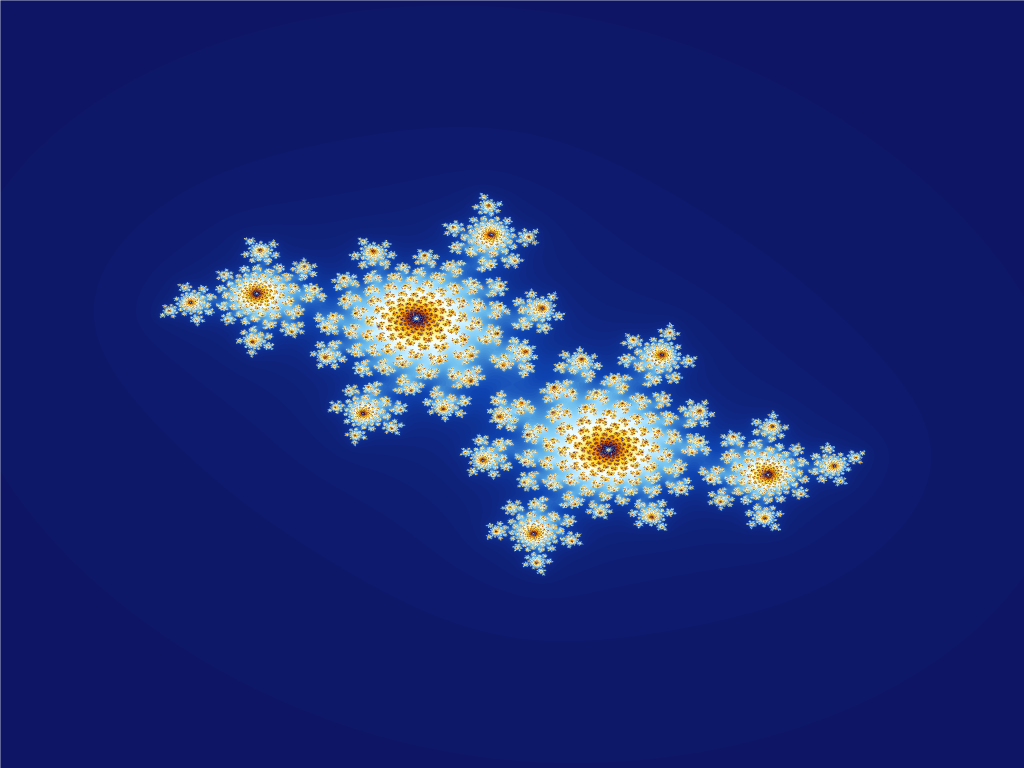
\includegraphics[width=200pt]{images/julia_wiki.png}
  \caption{The quadratic polynomial Julia set defined by \\$c=(\phi - 2)+(\phi - 1)i$ (from Wikipedia)}
\end{figure}

\section{Design}

\subsection{System Description and Development Environments}
\subsubsection{System Description}

The Interactive Fractal Generator is implemented on an \textbf{Altera DE2 Cyclone FPGA} by \textit{Terasic Technologies}. Terasic advertises the following specification about the device:

\begin{itemize}
\item Altera Cyclone II 2C35 FPGA with 35000 LEs
\item Altera Serial Configuration devices (EPCS16) for Cyclone II 2C35
\item USB Blaster built in on board for programming and user API controlling
\item JTAG Mode and AS Mode are supported
\item 8Mbyte (1M x 4 x 16) SDRAM
\item 512K byte(256K X16) SRAM
\item 4Mbyte Flash Memory (upgradeable to 4Mbyte)
\item SD Card Socket
\item 4 Push-button switches
\item 18 DPDT switches
\item 9 Green User LEDs
\item 18 Red User LEDs
\item 16 x 2 LCD Module
\item 50MHz Oscillator and 27MHz Oscillator for external clock sources
\item 24-bit CD-Quality Audio CODEC with line-in, line-out, and microphone-in jacks
\item VGA DAC (10-bit high-speed triple DACs) with VGA out connector
\item TV Decoder (NTSC/PAL) and TV in connector
\item 10/100 Ethernet Controller with socket.
\item USB Host/Slave Controller with USB type A and type B connectors.
\item RS-232 Transceiver and 9-pin connector
\item PS/2 mouse/keyboard connector
\item IrDA transceiver
\item Two 40-pin Expansion Headers with diode protection
\item DE2 Lab CD-ROM which contains many examples with source code to exercise the boards, including: SDRAM and Flash Controller, CD-Quality Music Player, VGA and TV Labs, SD Card reader, RS-232/PS-2 Communication Labs, NIOSII, and Control Panel API
\end{itemize}

\subsubsection{Development Environments}

\begin{itemize}
\item VHDL Development was done in the Altera Quartus II IDE v. 7.2
\item Software Development was done in a combination of Emacs v. 23.1 and the NIOS II IDE
\end{itemize}

\subsection{High-level Overview}


\begin{figure}\label{fig:block}
  \centering
	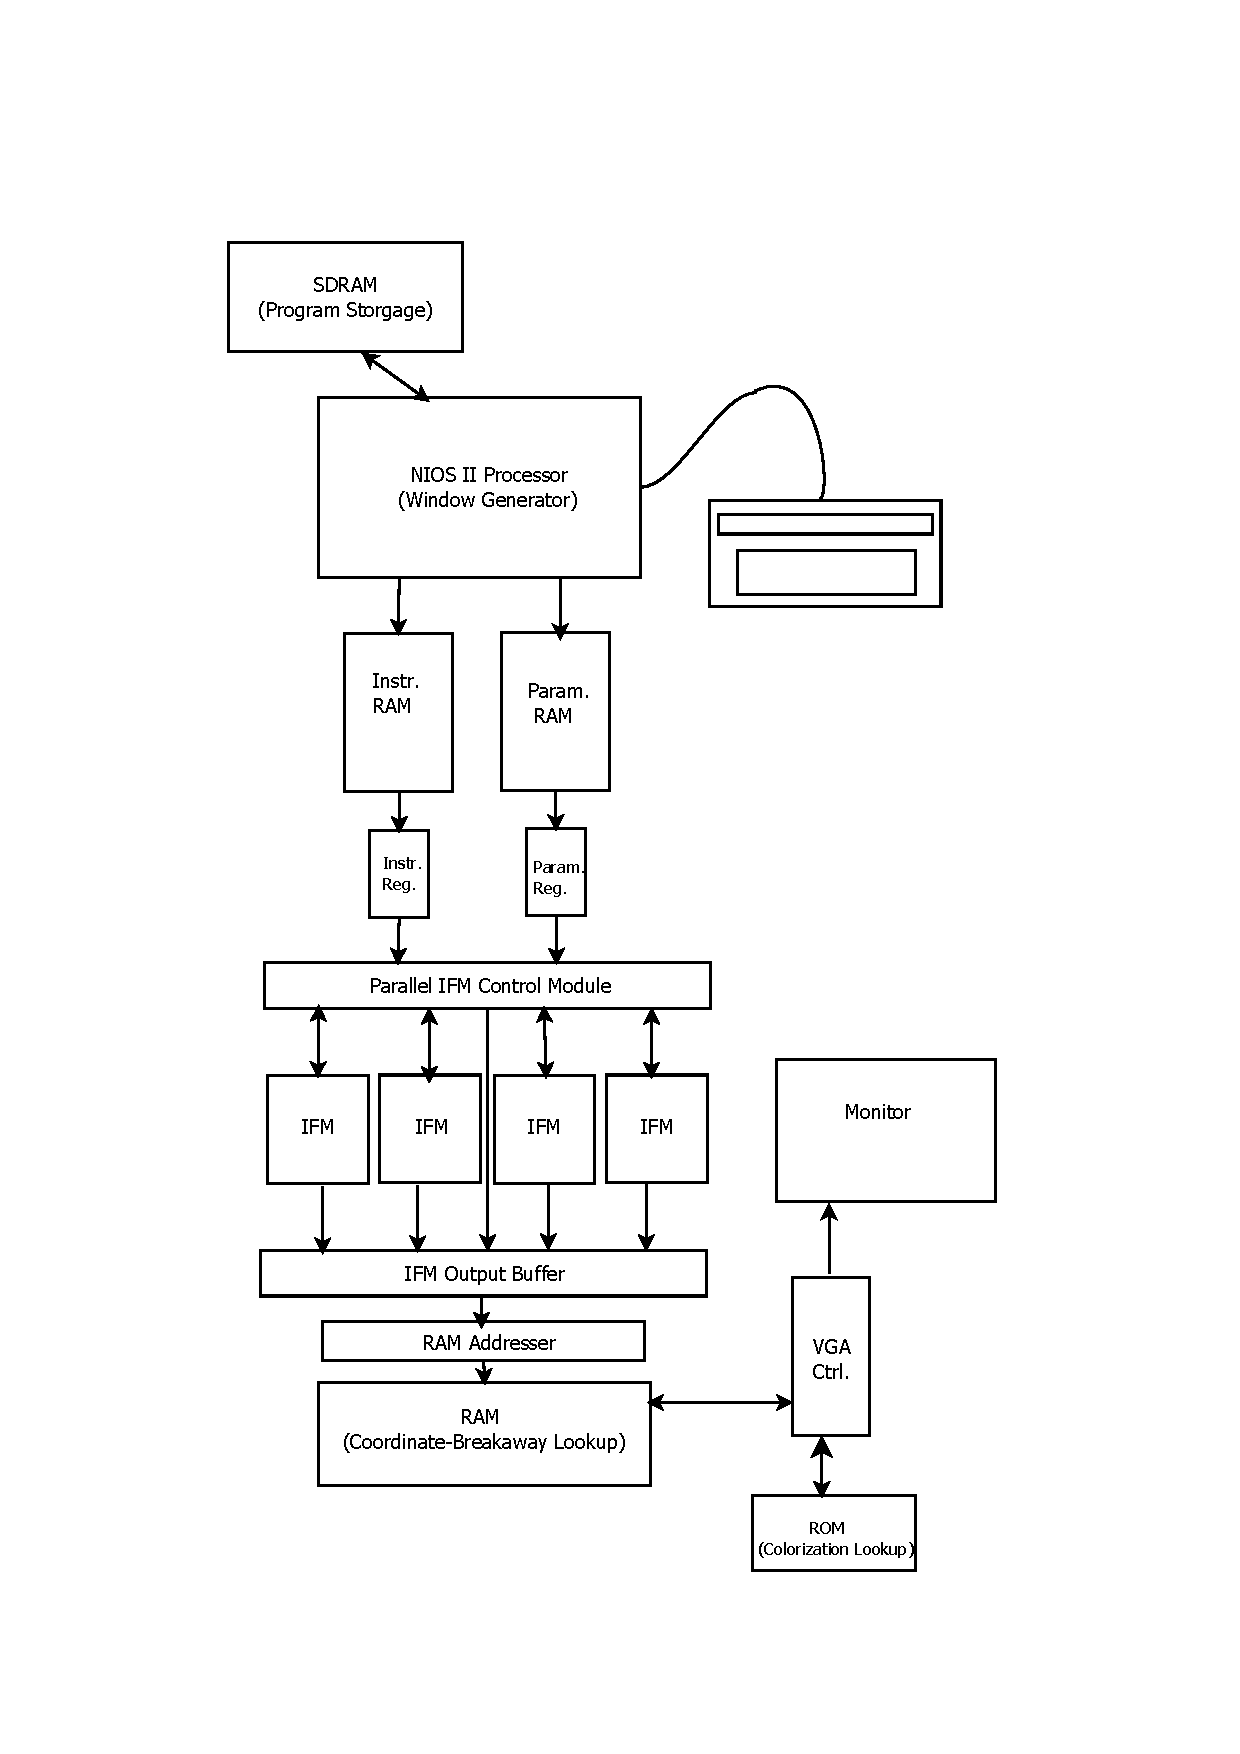
\includegraphics[width=\textwidth]{block_diagrams/juli_arch.pdf}
  \caption{High-level Block Diagram}
\end{figure}

The following is a description of how data travels through the block structure specified in Figure 2 when generating a single fractal.

\begin{itemize} 

\item Data flow originates from the \textbf{NIOS II Processor}, which initializes the system
by computing a set of parameters that can be used to describe the target window and 
fractal. The \textbf{NIOS} writes these parameters across the \textbf{Avalon Bus} onto an on-board \textbf{RAM} 
and sends instructions to generate a new image to a special instruction register.

\item When the instruction register receives the generate signal, it tells a component
charmingly referred to as the \texttt{Rammer} to write the parameters information contained 
in the \textbf{RAM} into registers. It then asserts a \textit{generate} signal that will be read by 
the \texttt{Window Generator}


\item The \texttt{Window Generator} takes these parameters as input and builds a set of 4-tuples $(x, y, a, b)$ where
  each tuple is a mapping from a \textbf{VGA} coordinate $(x, y)$ to a value in
  the complex plane of the form $a+bi$. The $(a, b)$ values eventually be used to compute a breakaway count $k$ for
  each co-ordinate on the screen. The computation will be performed by a specialized component called an 
  \texttt{Iterative Function Module}, or \texttt{IFM}.

\item Before the next $(a, b, x, y)$ tuple is delivered to one of the $4$ available \texttt{IFM}s, it must be requested by a component
known as the \texttt{IFM Controller}. The \texttt{IFM Controller} is responsible for distributing work among
several \texttt{IFM}s working in parallel. 

\item When an \texttt{IFM} enters a ready state, it is given the next $(a, b, x, y)$ tuple and will begin performing
the function iterations using the constant prescribed by the set to be generated. The \texttt{IFM} transitions into a 
done state after a fixed number of iterations, or when the squared magnitude of its current iteration exceeds $4$.

\item The \texttt{IFM Controller} takes the data given by the done-state \texttt{IFMs} and writes it to a queue
that will deliver it to the \texttt{Coordinate-Breakaway Lookup Table}, implemented using the on-board \textbf{SRAM}. 
The \texttt{IFM} data takes the form of the $(x, y, k)$ triples we set out to create. The $k$ value of each triple
is stored in the \texttt{Coordinate-Breakaway Lookup Table} at an address determined by the $(x, y)$ values. In this 
way, we map \textbf{VGA} coordinates to their associated breakaway iterations.

\item The \texttt{VGA Module} fetches results from the \texttt{Coordinate-Breakaway
  Lookup Table} and colorizes them using a separate \textbf{ROM}-based \texttt{Colorization Lookup Table}.
  The \texttt{Colorization Lookup Table} takes a breakaway count, $k$, and maps it to an $(r, g, b)$ bit-vector for use by the \textbf{VGA}.
\end{itemize}


% ------------------------------------------------------------
% now, we delve into the lower levels of the implementation
% ------------------------------------------------------------
\subsection{Module Implementation}

% ----------------------------------------
\subsubsection{User Interface Module}

As an interactive device, our fractal generator has the capacity to accept user parameters such as window size or
Julia set constants during operation. This communication with the user is facilitated by the NIOS II Processor 
taking PS/2 keyboard input. We refer to these entities and all their supporting devices as the \texttt{User Interface 
Module}. This module is responsible for handling communication with input peripherals
and translating user input into information that can easily be used by the hardware-based fractal generator. Once 
this information has been translated into a set of values that can be used by the remainder of the system generator, they are written into an on-board RAM. When the \texttt{User Interface Module} is ready for the hardware to take some action, it sends a signal to a component on the board, which forwards the signal appropriately. All communication with
the board is performed over the Avalon Interconnect Fabric.

The NIOS II Processor uses the SDRAM as its memory store.

\begin{figure}
  \centering
    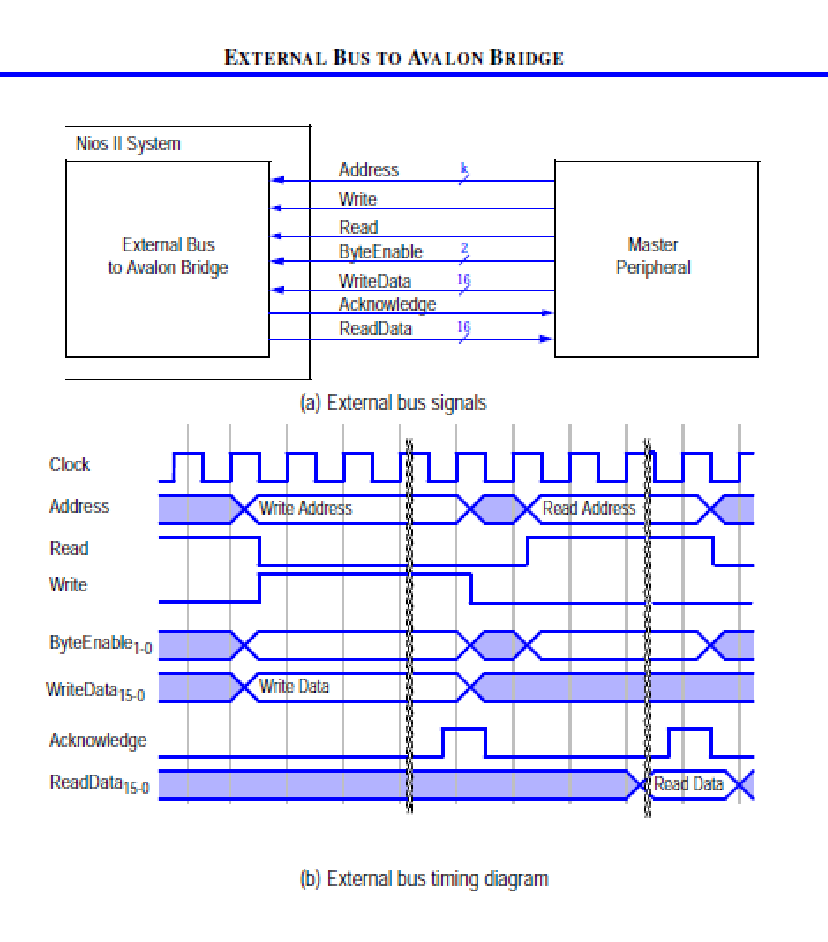
\includegraphics[width=200pt]{block_diagrams/nbat.pdf}
  \caption{Block and Timing Diagram of the Avalon interconnect fabric. Provided by Altera Corporation.}
\end{figure}

Parameters of primary concern are those of viewing window and Julia set constant. The window is set using the 
following values (which will be elaborated on in the \texttt{Window Generator} section):

\begin{tabular}{rll}
-&$a_{min}$ & $36$ bits\\
-&$a_{diff}$ & $36$ bits\\
-&$a_{leap}$ & $10$ bits\\
-&$b_{min}$ & $36$ bits\\
-&$b_{diff}$ & $36$ bits\\
-&$b_{leap}$ & $10$ bits\\
\end{tabular}

Meanwhile, the Julia set constant is set using the following values

\begin{tabular}{rll}
-&$c_{real}$ & $36$ bits\\
-&$c_{img}$ & $36$ bits
\end{tabular}

\subsubsection{Parameter RAM}
In order to allow for the buffering and mutation of individual parameters, the \texttt{UI Module} writes each 
individual parameter into a RAM. Since the Avalon interconnect fabric only allows for $32$ bits to be transferred
at once, but most parametrs are $36$ bits wide, the RAM is $18$ bits in width and parameters are sent in with the
$18$ least significant bits of each $32$ bit write. For simplicity, these rows are still addressed by the 
NIOS as if they were $32$ bits wide.

Each of the $14$ rows in this RAM has a different purpose.

\begin{tabular}{rlcl}
\textbf{Row}&\textbf{Data Stored}&\textbf{Portion}&\textbf{Offset}\\ \hline
0&$a_{min}$ &18 MSB& 0x0\\
1&$a_{min}$ &18 LSB& 0x4\\
2&$b_{min}$ &18 MSB& 0x8\\
3&$b_{min}$ &18 LSB& 0xC\\
4&$a_{diff}$ &18 MSB& 0x10\\
5&$a_{diff}$ &18 LSB& 0x14\\
6&$b_{diff}$ &18 MSB& 0x18\\
7&$b_{diff}$ &18 LSB& 0x1C\\
8&$a_{leap}$ &-& 0x20\\
9&$b_{leap}$ &-& 0x24\\
10&$c_{real}$ &18 MSB& 0x28\\
11&$c_{real}$ &18 LSB& 0x2C\\
12&$c_{img}$ &18 MSB& 0x30\\
13&$c_{img}$ &18 LSB& 0x34\\
\end{tabular}

When the \texttt{UI Module} sends a redraw signal to the board, a device called the \texttt{Rammer} moves
these values into registers that will be read by the \texttt{Window Generator} and \texttt{IFM}s when drawing
the image.

\subsubsection{Window Generator}

The \texttt{Window Generator} serves to kick off the calculation cascade,
computing the position in the complex plane represented by each pixel in the
given input window, thereby producing 
$(x, y, a, b)$ tuples. 

\begin{figure}
  \centering
    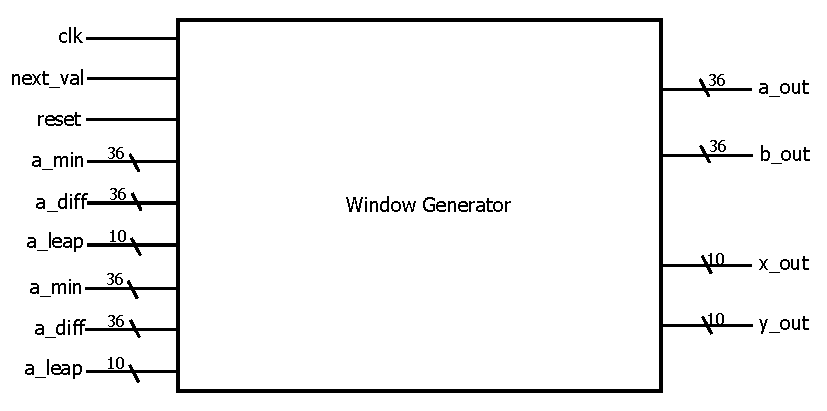
\includegraphics[width=240pt]{block_diagrams/win_gen.pdf}
  \caption{High-level Block Diagram of the Window Generator}
\end{figure}


The generator uses a specialized procedure that requires only addition and comparison
operations to map out a whole window. Say we have a window that stretches from $v_{min}$ to $v_{max}$ over
N pixels. The procedure works by iterating from 0 to N-1 and producing a sum at each step of the way that
corresponds to a the value of $v$ at that point. The procedure requires a few values as input:

\begin{tabular}{rl|p{10cm}}
\textbf{Parameter}&\textbf{Width}&\textbf{Purpose}\\
&&\\
$a_{min}$ & 36 bits& Describes the minimum value of $a$ in the window\\
&&\\
$a_{diff}$ & 36 bits& Describes the standard differential between consecutive a values in the window $(a_{max} - a_{min})/WIDTH_{SCREEN}$ this is computed by the NIOS processor.\\
&&\\
$a_{leap}$ & 10 bits& Periodically, we will need to add 1 to our sum to compensate for precision loss. This value
corresponds to the length of the intervals between these ``leap cycles'' $WIDTH_{SCREEN}/((a_{max} - a_{min}) \mod WIDTH_{SCREEN})$\\
&&\\
$b_{min}$ & 36 bits& Describes the minimum value of $a$ in the window.\\
&&\\
$b_{diff}$ & 36 bits& Describes the standard differential between consecutive a values in the window $(b_{max} - 
b_{min})/HEIGHT_{SCREEN}$ this is computed by the NIOS processor.\\
&&\\
$b_{leap}$ & 10 bits& Periodically, we will need to add 1 to our sum to compensate for precision loss. This value
corresponds to the length of the intervals between these ``leap cycles'' $HEIGHT_{SCREEN}/((b_{max} - b_{min}) \mod HEIGHT_{SCREEN})$\\
&&\\
\end{tabular}

The \texttt{Window Generator} is therefore comprised of two \texttt{Differential Counters} that are responsible for performing the 
iterations. One computes values for $b$ and the other $a$. 

\begin{figure}
  \centering
    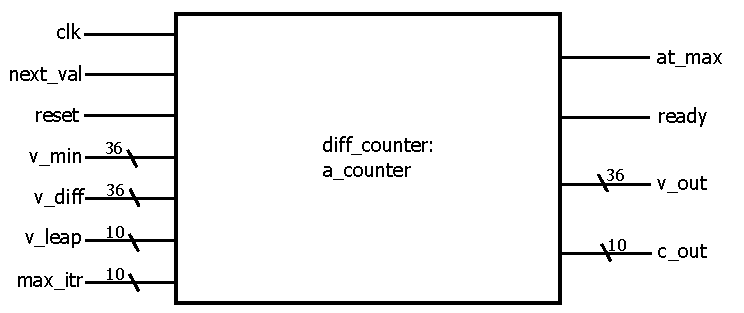
\includegraphics[width=240pt]{block_diagrams/acounter.pdf}
  \caption{Block diagram of a \texttt{Differential Counter} used in window generation}
\end{figure}

When the \texttt{Differential Counter} receives a reset signal, it initializes its data according to the signals coming in.
Then, each time it recieves a next-value signal, it increments the output value accordingly. If the counter reaches
its maximum, it asserts a flag.

\begin{figure}
  \centering
    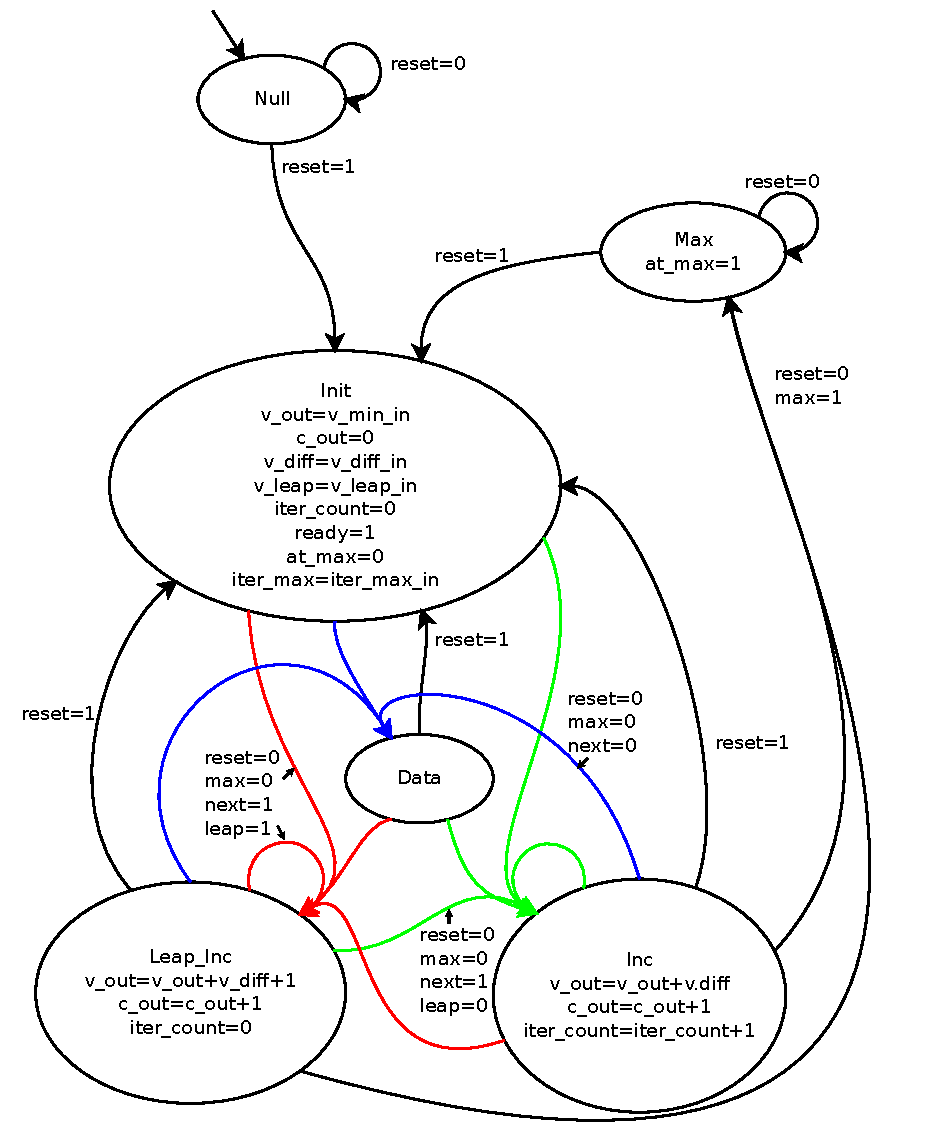
\includegraphics[width=300pt]{state_diagrams/diff_counter.pdf}
  \caption{State Diagram for the \texttt{Differential Counter}, Moore machine: signals
    \texttt{max=c\_cuis=max\_itr}, \texttt{leap=iter\_count=v\_leap}. Omit
    unused signals (X) for compactness. Colorcoded signal bundles.}
\end{figure}

\begin{figure}
  \centering
    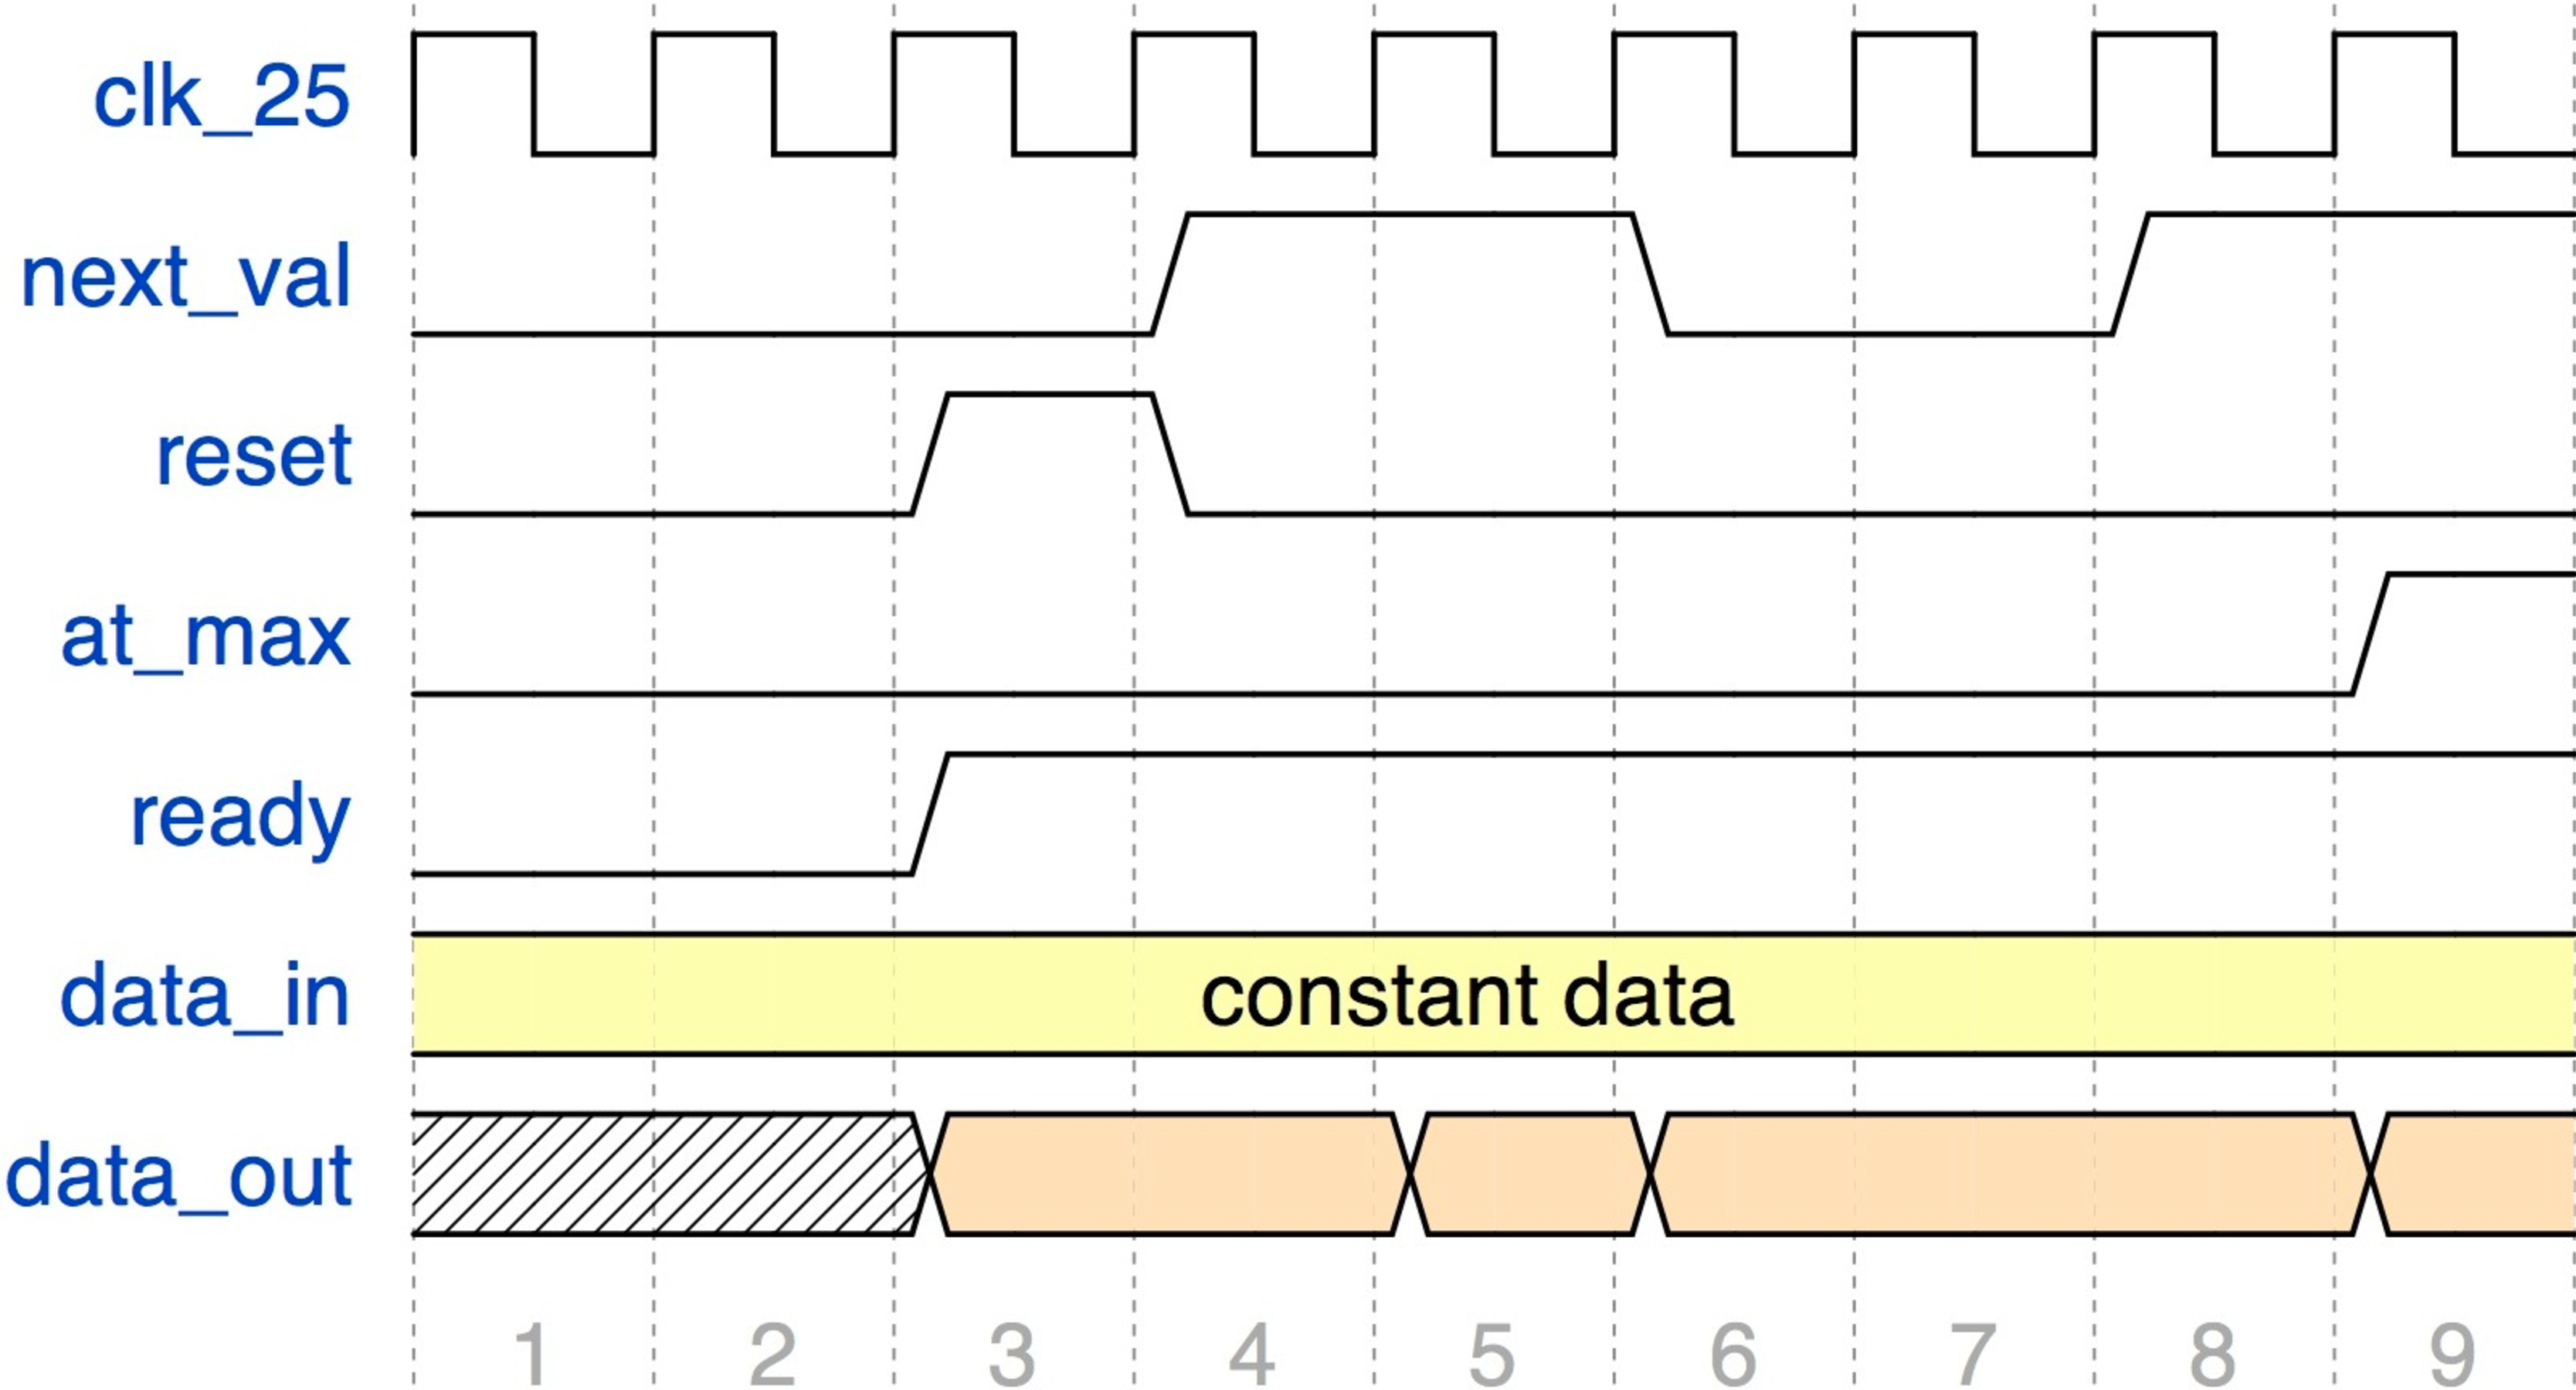
\includegraphics[width=300pt]{timing_diagrams/diff_counter.pdf}
  \caption{Timing diagram of the \texttt{Differential Counter}}
\end{figure}

In the \texttt{Window Generator}, the \texttt{Differential Counters} are hooked up in such a way that the points are cycled through
from left to right down the screen.

\begin{figure}
  \centering
    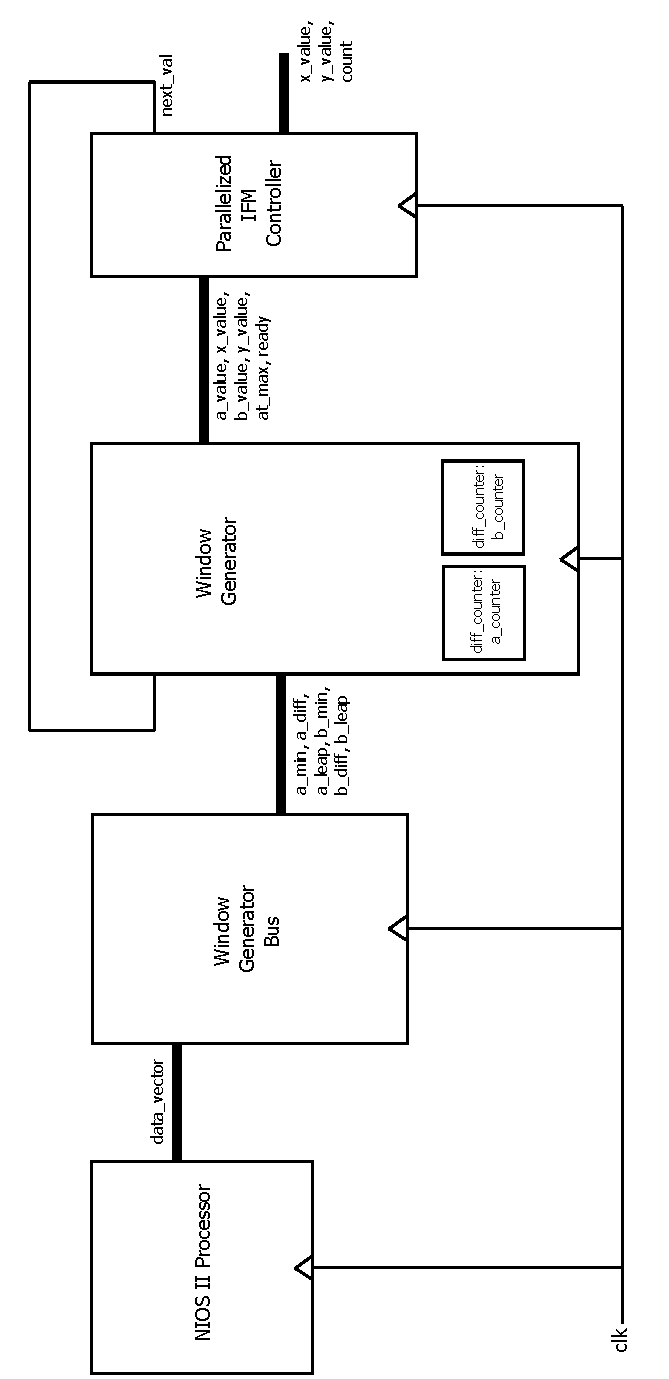
\includegraphics[width=250pt, angle=270]{block_diagrams/win_gen_interior.pdf}
  \caption{Block diagram illustrating $(x, y, a, b)$ tuple dataflow.}
\end{figure}

The \texttt{Window Generator} takes reset signals from the bus connected to the NIOS processor. When the \texttt{Window
Generator} is ready for computation (the same cycle that it is reset by the bus), it asserts a data flag.
When the \texttt{IFM} reads an $(x, y, a, b)$ tuple, it asserts a next value signal indicating that it will need new data in the following cycle. Once the \texttt{Window Generator} runs out of values to give, it asserts an at max flag.

\begin{figure}
  \centering
    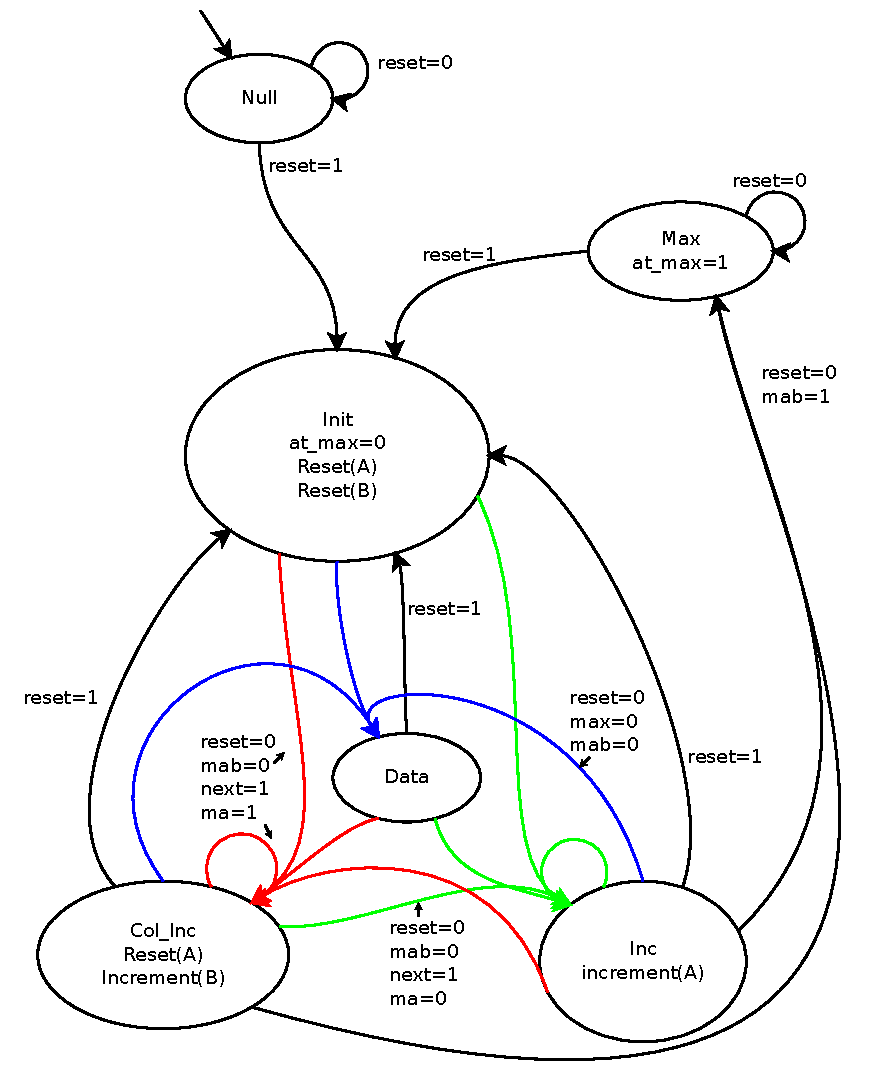
\includegraphics[width=180pt]{state_diagrams/diff_window_gen.pdf}
  \caption{State Diagram for the \texttt{Window Generator} code, Moore machine:
    signals \texttt{max=c\_cuis=max\_itr},
    \texttt{leap=iter\_count=v\_leap}. Omit unused signals (X) for
    compactness.}
\end{figure}


\begin{figure}
  \centering
    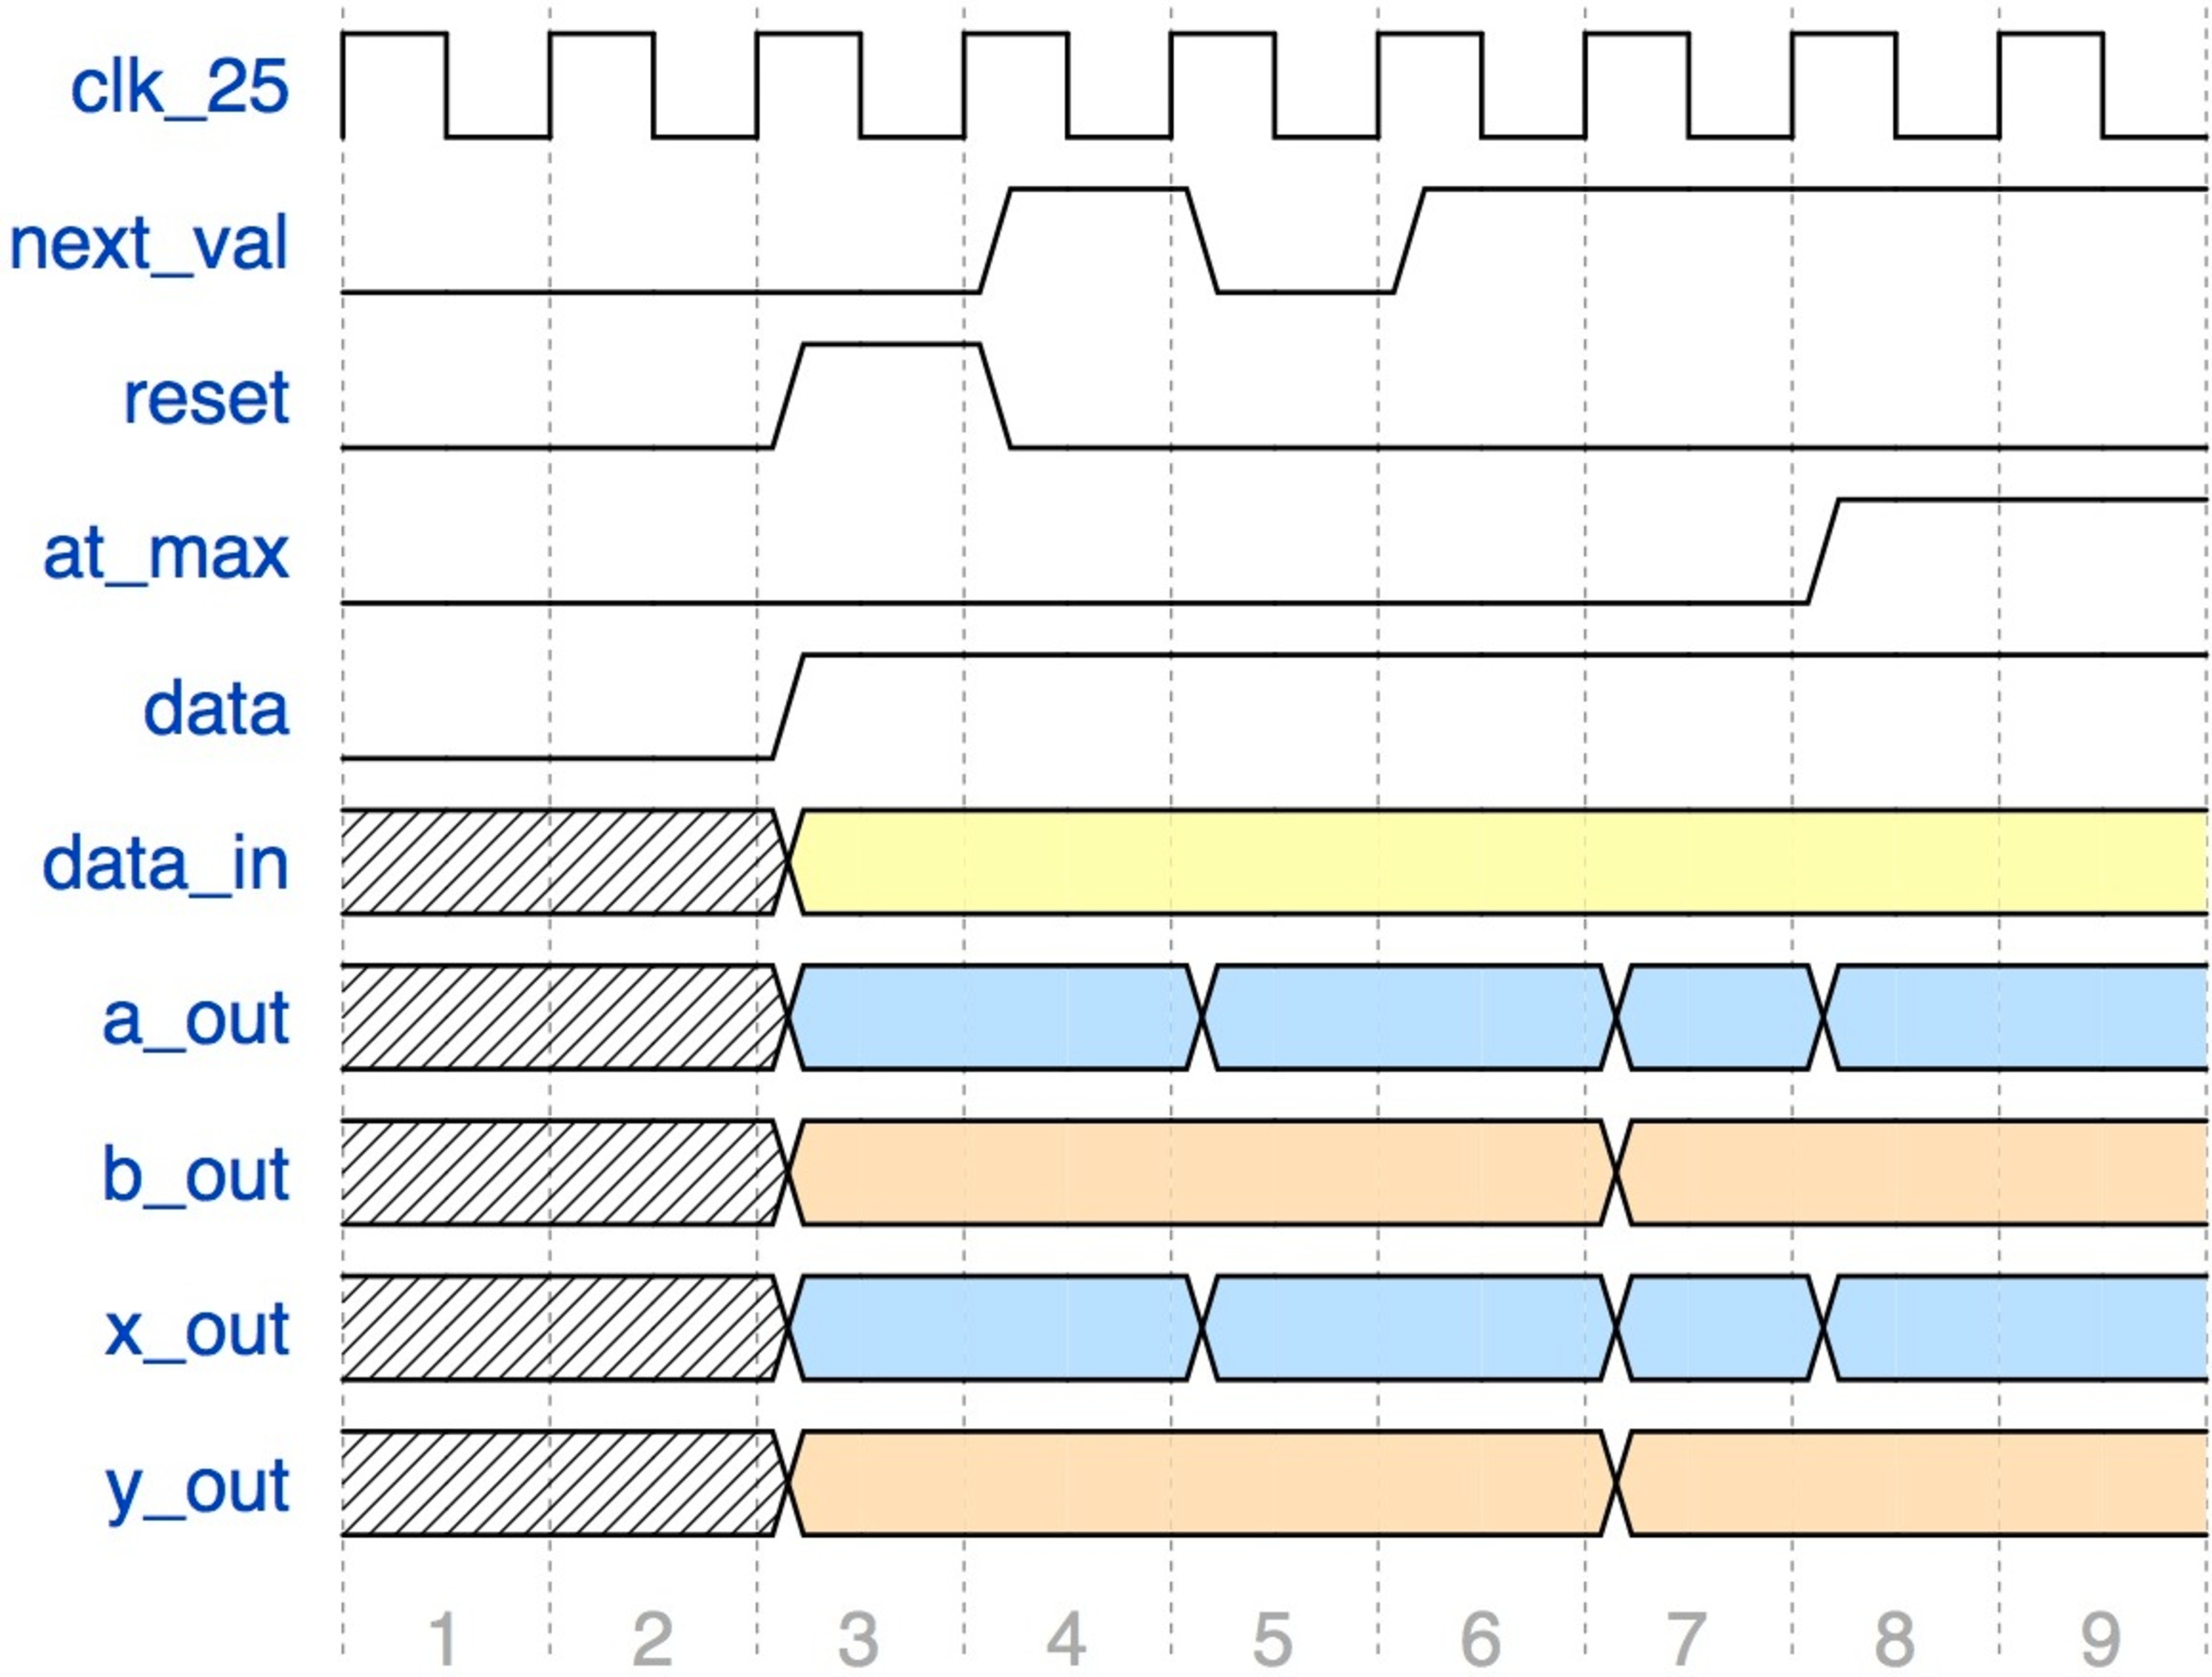
\includegraphics[width=240pt]{timing_diagrams/gen_ifm.pdf}
  \caption{Timing diagram of interface between the \texttt{Window Generator}
    and the IFMs.}
\end{figure}

\subsubsection{IFM Controller}

Rendering Julia set fractals requires many iterations of relatively
simple computations in the complex plane. This sequence of
computations is independent for each point in the image, which is why
the calculation of fractal sets lends itself to parallel
computation. However, the very nature of the iterated fractal
calculation means that the amount of time spent performing computations on each individual point
can vary drastically, introducing synchronization issues. It is the responsibility of the
\texttt{IFM Controller} to resolve these issues.

\begin{figure}
  \centering
    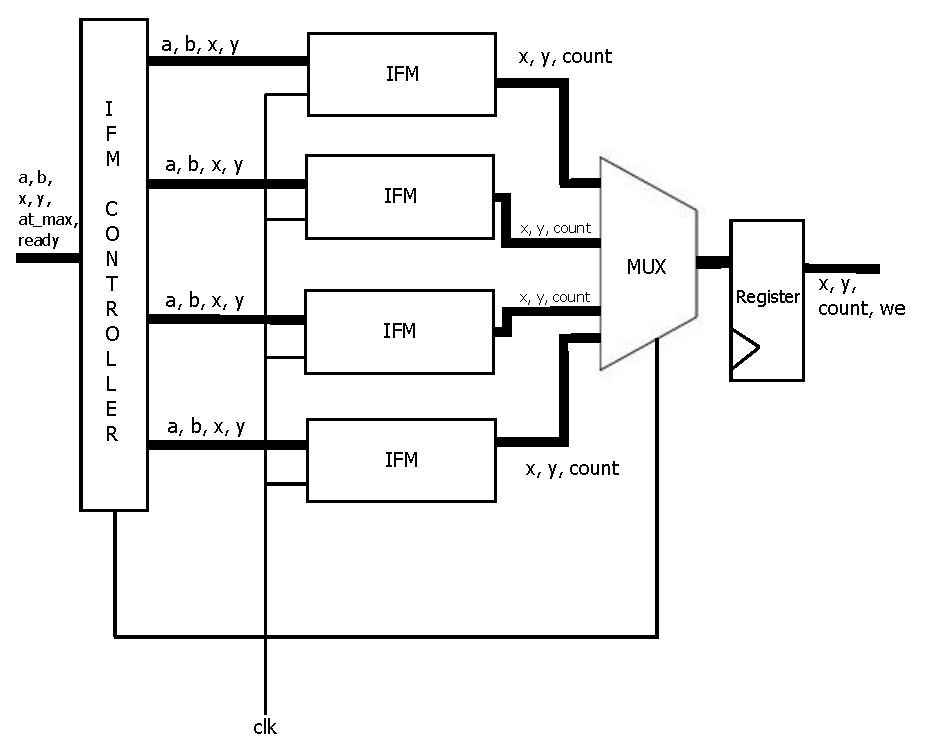
\includegraphics[width=240pt]{block_diagrams/ifmunit.pdf}
  \caption{Block diagram for the IFM wrappers}
\end{figure}


The \texttt{IFM Controller} constantly transmits the $(x, y, a, b)$ tuple currently being expressed by the window generator to each of the \texttt{IFM}s. When an \texttt{IFM} indicates that it is in the ready state, the controller asserts a signal instructing the 
\texttt{IFM} to accept the new data and begin computation (assuming that the window generator is asserting the valid data flag).
Simultaneously, the controller signals to the \texttt{Window Generator} that it needs the next data tuple in the window. If more
than one \texttt{IFM} is in the ready state at once, the controller only sends the read and compute signal to one, saving the upcoming data tuples for the rest.


% ----------------------------------------
\subsubsection{Iterative Function Module (IFM)}

A quadratic polynomial Julia set is generated by applying the function

\begin{equation}
f_c(z) = z^2 + c
\end{equation}

repeatedly, where $z,c \in \mathbb{C}$. For any given pair $(z, c)$, this recurrence will result in one of two outcomes:
\begin{itemize}
\item The magnitude of the complex values generated by the recurrence may stay bounded by $2$
\item The magnitude may become unbounded and escape toward infinity
\end{itemize}

A point $z$ on the complex plane is in the Julia set uniquely defined by the complex number $c$ if and only if the 
recurrence remains bounded for $(z, c)$. To determine whether or not a point remains bounded for a given $c$, we compute
a fixed number of iterations on the recurrence (in our case $127$) and report the iteration in which the value generated has
a squared magnitude of greater than $4$. Those points that do not become unbounded in this many iterations are considered
to be part of the set.

Because the factors of the multiplication are complex numbers, computing their product involves
$3$ real-number multiplications. For $z = a + bi$ we compute\\

\begin{eqnarray}
P_A &=& a^2 \nonumber \\
P_B &=& b^2 \nonumber \\
P_C &=& ab \nonumber
\end{eqnarray}

With these values we can compute:

\begin{eqnarray}
a_{next} &=& P_A - P_B + c_{real}\nonumber \\
b_{next} &=& 2P_C - c_{img} \nonumber \\
|z|^2 &=& P_A + P_B \nonumber 
\end{eqnarray}

The squaring operations for $P_A$ and $P_B$ is perfomed by a specialized logical circuit provided as an \textit{Altera Megafunction}. The multiplication $P_C$ is perfomed by embedded multipliers on the DE2. These are expansive circuits, but the FPGA is still to accomodate up to $4$ \texttt{IFM}s.

\begin{figure}[H]
  \centering
    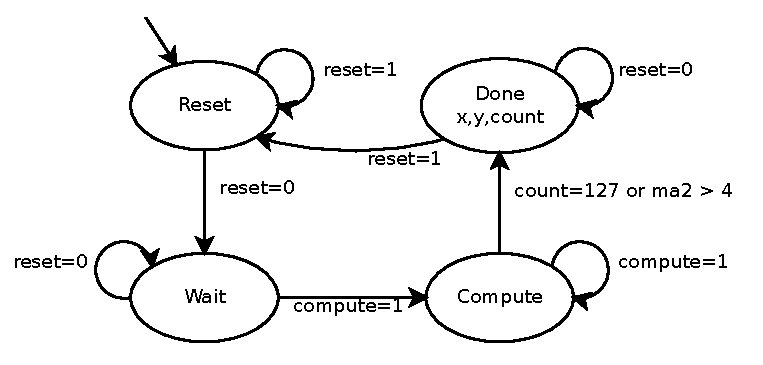
\includegraphics[width=300pt]{state_diagrams/ifm.pdf}
  \caption{State diagram for a single \texttt{IFM}. Moore
    machine: using abstract transition descriptions. Omits unused
    signals for compactness.}
\end{figure}


\begin{figure}[H]
  \centering
    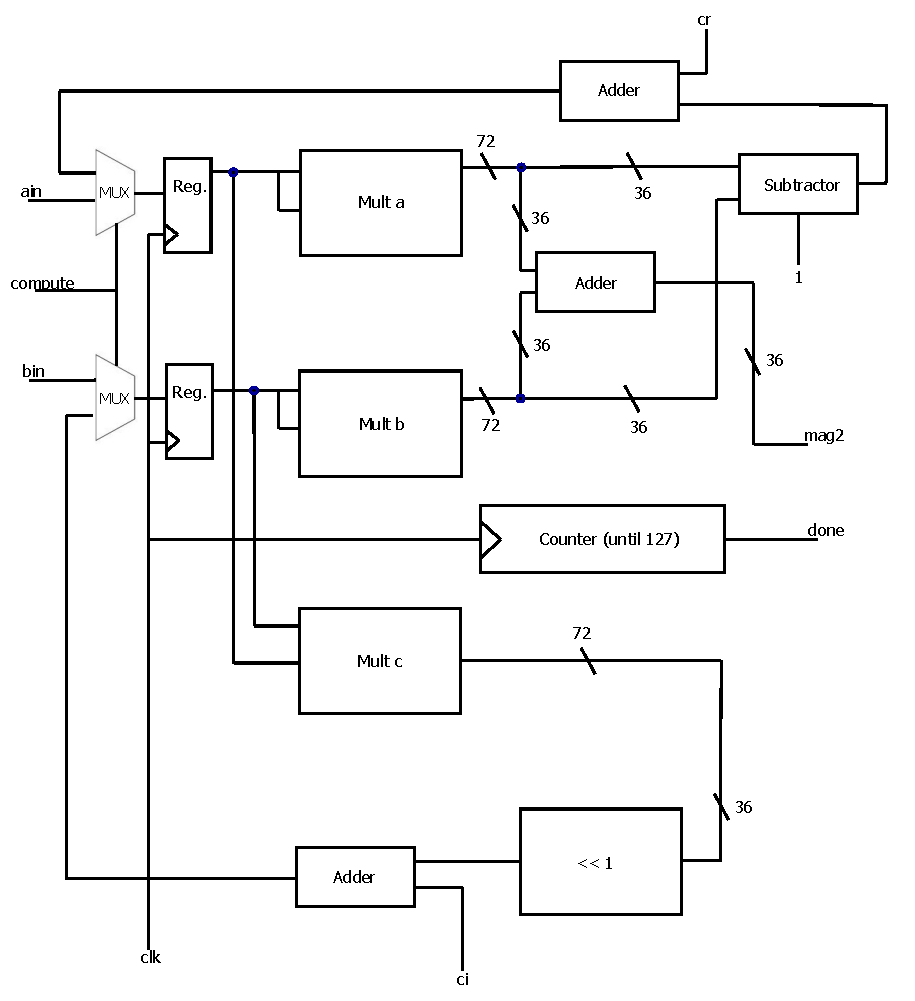
\includegraphics[width=240pt]{block_diagrams/ifm.pdf}
  \caption{Arithmetic Logic Circuit within each \texttt{IFM}}
\end{figure}

Real-valued numbers are represented as two's-complement fixed-point binary
values in our circuit. A complex number is comprised of two such data vectors. 
We restrict ourselves to 36 bits, as the onboard multipliers
are sized as such. 

In order to accomodate the largest-magnitude value we
expect to come across during any iteration, we require 6 bits to the
left of the radix. Thus, our fixed-point values have 30 bits to the
right of the radix. This gives us a machine precision of approximately
$9.31 \times 10 ^ {-10}$.

\begin{figure}[H]
  \centering
    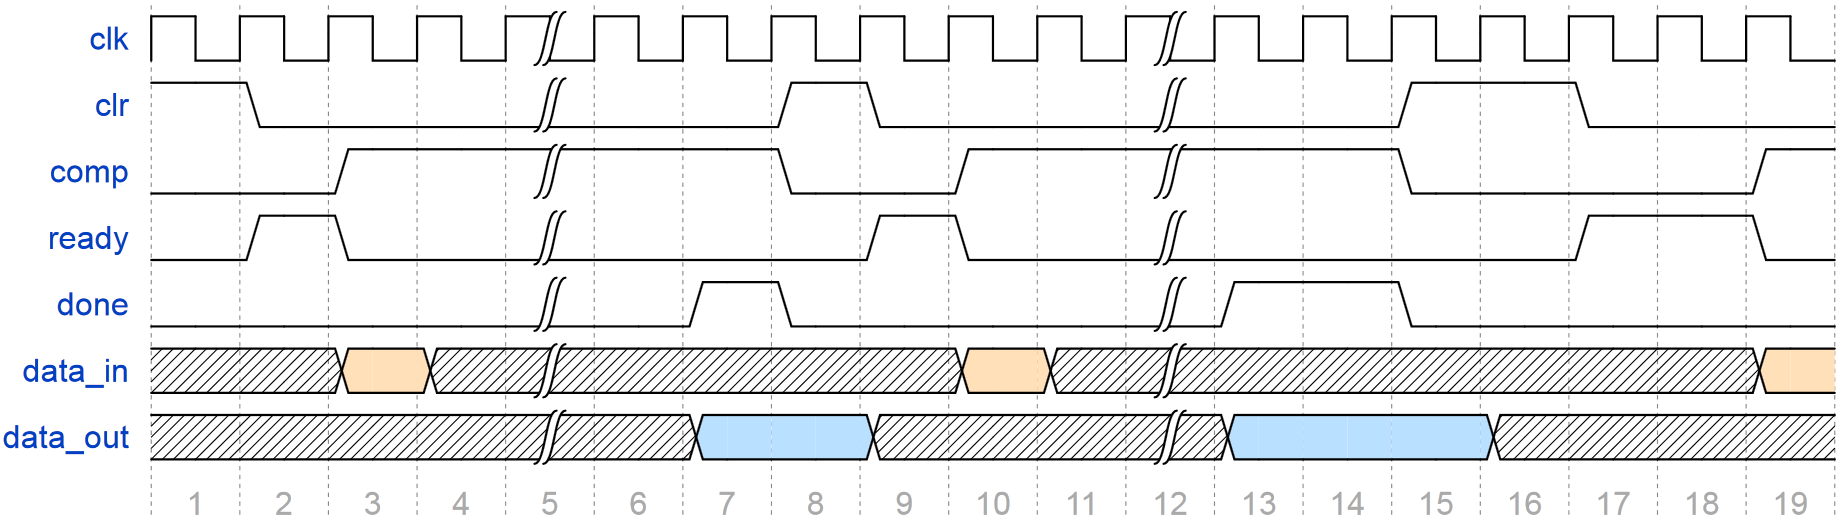
\includegraphics[width=300pt]{timing_diagrams/IFM.PNG}
  \caption{Timing diagram for a single \texttt{IFM}.}
\end{figure}


To more easily facilitate communication with the \texttt{IFM Controller}, each \texttt{IFM} is contained within a wrapper module.
Thus, the \texttt{IFM Controller} need only alter the state of the wrapper module, and the wrapper module will transmit signals to the \texttt{IFM}s indicating the desired behavior.

\begin{figure}[H]
  \centering
    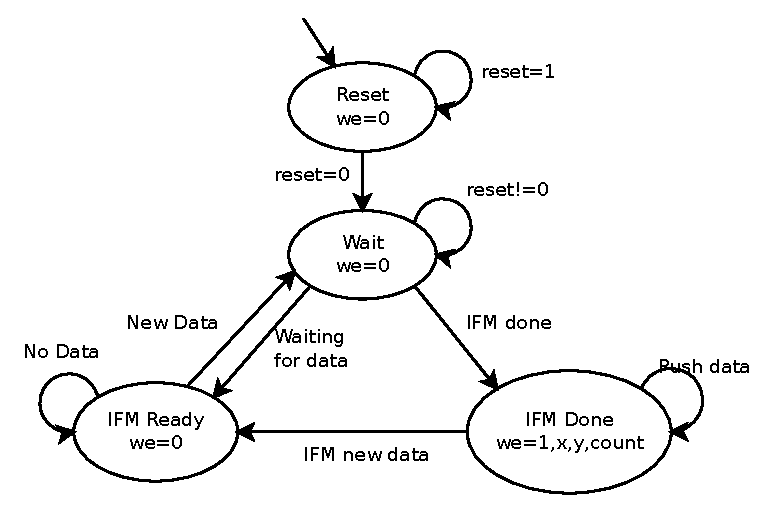
\includegraphics[width=300pt]{state_diagrams/ifmunit.pdf}
  \caption{State diagram for a single \texttt{IFM} wrapper module,
    Moore machine: using abstract transition descriptions.}
\end{figure}

If a wrapper module is in the done state, the controller indicates that its $(x, y, c)$ triple should be read into
the output register. If multiple \texttt{IFM} wrappers are in the done state simultaneously, the controller chooses one at a
time to be read in. These triples are then augmented with an asserted write enable flag to indicate that they represent
valid data, and should be written to the \texttt{Coordinate-Breakaway lookup table}. 


% ----------------------------------------
\subsubsection{Coordinate-Breakaway Lookup Table}

After the count associated with each pixel is calculated, it must be
stored in a framebuffer that interfaces both with the \texttt{IFM
Controller} as well as the \texttt{VGA Module}.

\begin{figure}[H]
  \centering
    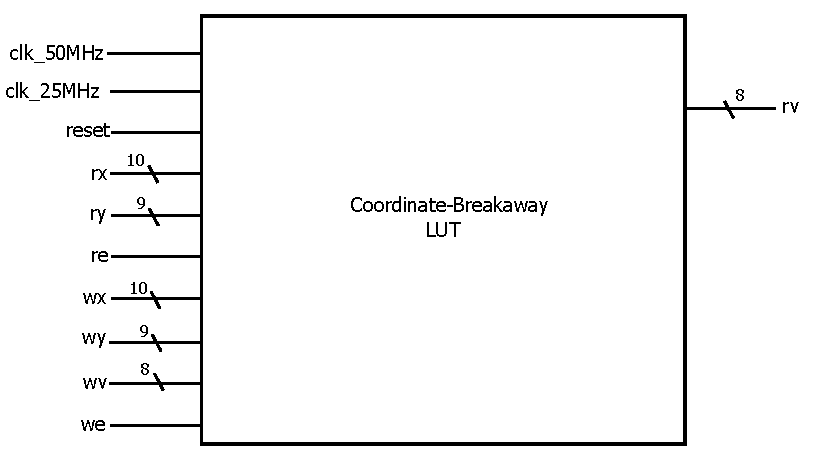
\includegraphics[width=240pt]{block_diagrams/clut.pdf}
  \caption{Block Diagram of the \texttt{Coordinate-Breakaway LUT}: signals on
    the right side are inputs, signals on the left are outputs.}
\end{figure}

For this, we use the SRAM chip that is built into the DE2 board, for
its relatively expansive memory size (versus on-chip memory), fast
speed, and ease of use (versus the SDRAM chip). The SRAM chip has a 
512kibibytes capacity that can be accessed and written to in half a 50MHz
clock cycle, making it ideal for our purposes.

Since we display a $640\times 480$ image in the VGA module and keep 8
bits of iteration information for each pixel, we need a grand total of
300kibibytes to store the information, fitting well within the
confines of the given 512kibibyte SRAM chip.

We use a straightforward addressing scheme to store the count
information, using the $y$ position as the top 9 bits of the address,
and the $x$ position as the bottom 10 bits of the address. This way,
finding the address from a given pixel position is very fast.

A small wrinkle is the fact the SRAM is in fact a $256K\times 16$ bit memory,
reading and writing in 16 bit chunks. This merely means that the very
bottom bit of the $x$ position does not go to the address, but is
routed to the bitmask signal indicating whether the byte sought is in the upper or lower half.
Of the 16-bit word that is addressed by the remaining 18 bits.

\paragraph{Reading/Writing}

Since the SRAM has only one IO port, reads and writes must be time
multiplexed. The VGA module will be consistently requesting data from the SRAM at 25MHz. However, while 
the fractal is being generated, the IFMs will be providing information that must be written to the SRAM 
at the same frequency. This means that we must interleave reads and writes to the SRAM.

We can use the structure of the reads from the VGA to our
advantage to make room for the necessary writes. Reads always follow a pattern, where
if we read the lower half of a 16bit word, then we will read the
higher half in the next 25MHz clock cycle. Hence, when we require the lower
half of a word, we can fetch the entire word in one read, save the
higher half in a register, and return it when it's required in
the next clock cycle. In this way, we reduce the frequency of VGA reads from the SRAM to every other cycle on a 
25MHz clock.

\begin{figure}[H]
  \centering
    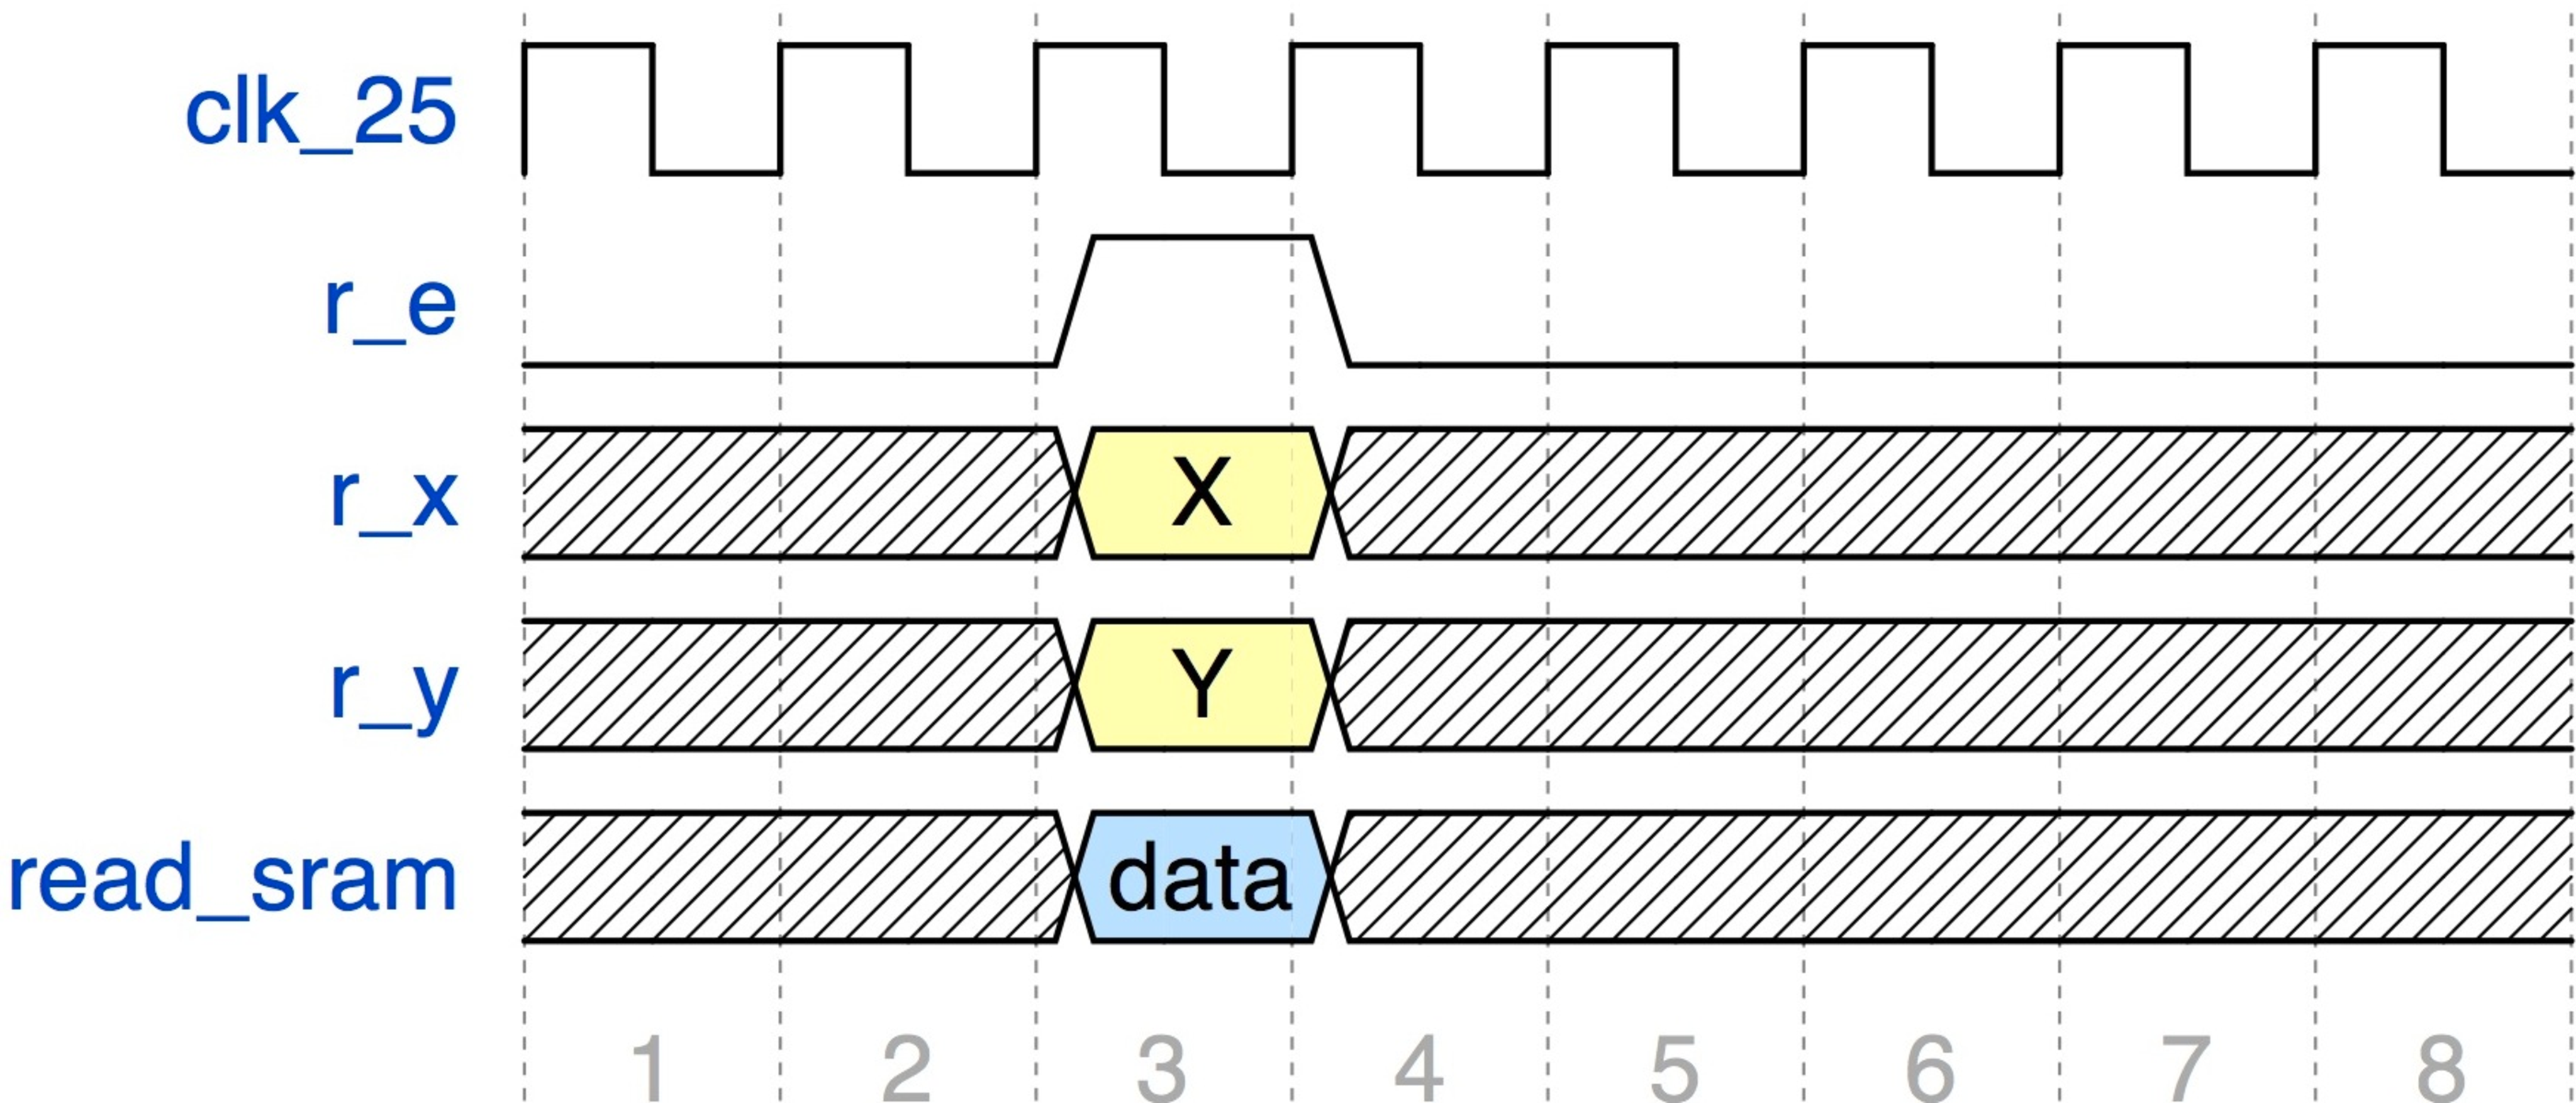
\includegraphics[width=300pt]{timing_diagrams/clut_vga.pdf}
  \caption{Timing diagram of the interface between the Coordinate-Breakaway LUT and VGA module}
\end{figure}

Even with every other 25Mhz cycle being dedicated to writing the data being sent out by the \texttt{IFM}s, the SRAM might
still miss a coordinate if the \texttt{IFM}s are generating their maximum possible throughput of 25MB/s. To account for this, 
we prioritize writes over reads. Even if a VGA read is missed in one scan, it will be correct in the next scan as long as writes are prioritized. The junction writing to the SRAM consists of a shift register that 
constantly reads from the \texttt{IFM} output, but only shifts when the SRAM's read enable signal is not being asserted. 

\begin{figure}[H]
  \centering
    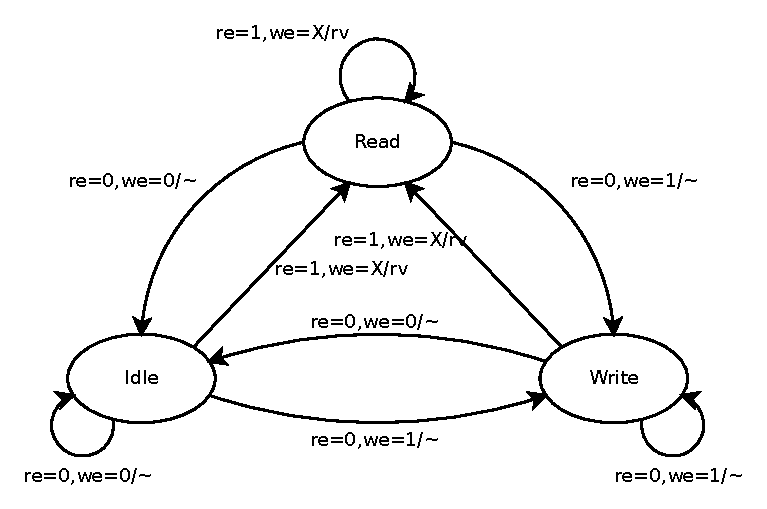
\includegraphics[width=300pt]{state_diagrams/clut.pdf}
  \caption{Simplified State Diagram of the \texttt{Coordinate-Breakaway LUT}:
    Mealy machine, only includes re and we as inputs and rv as an
    output, with $\thicksim$ denoting a lack of outputs}
\end{figure}

\begin{figure}[H]
  \centering
    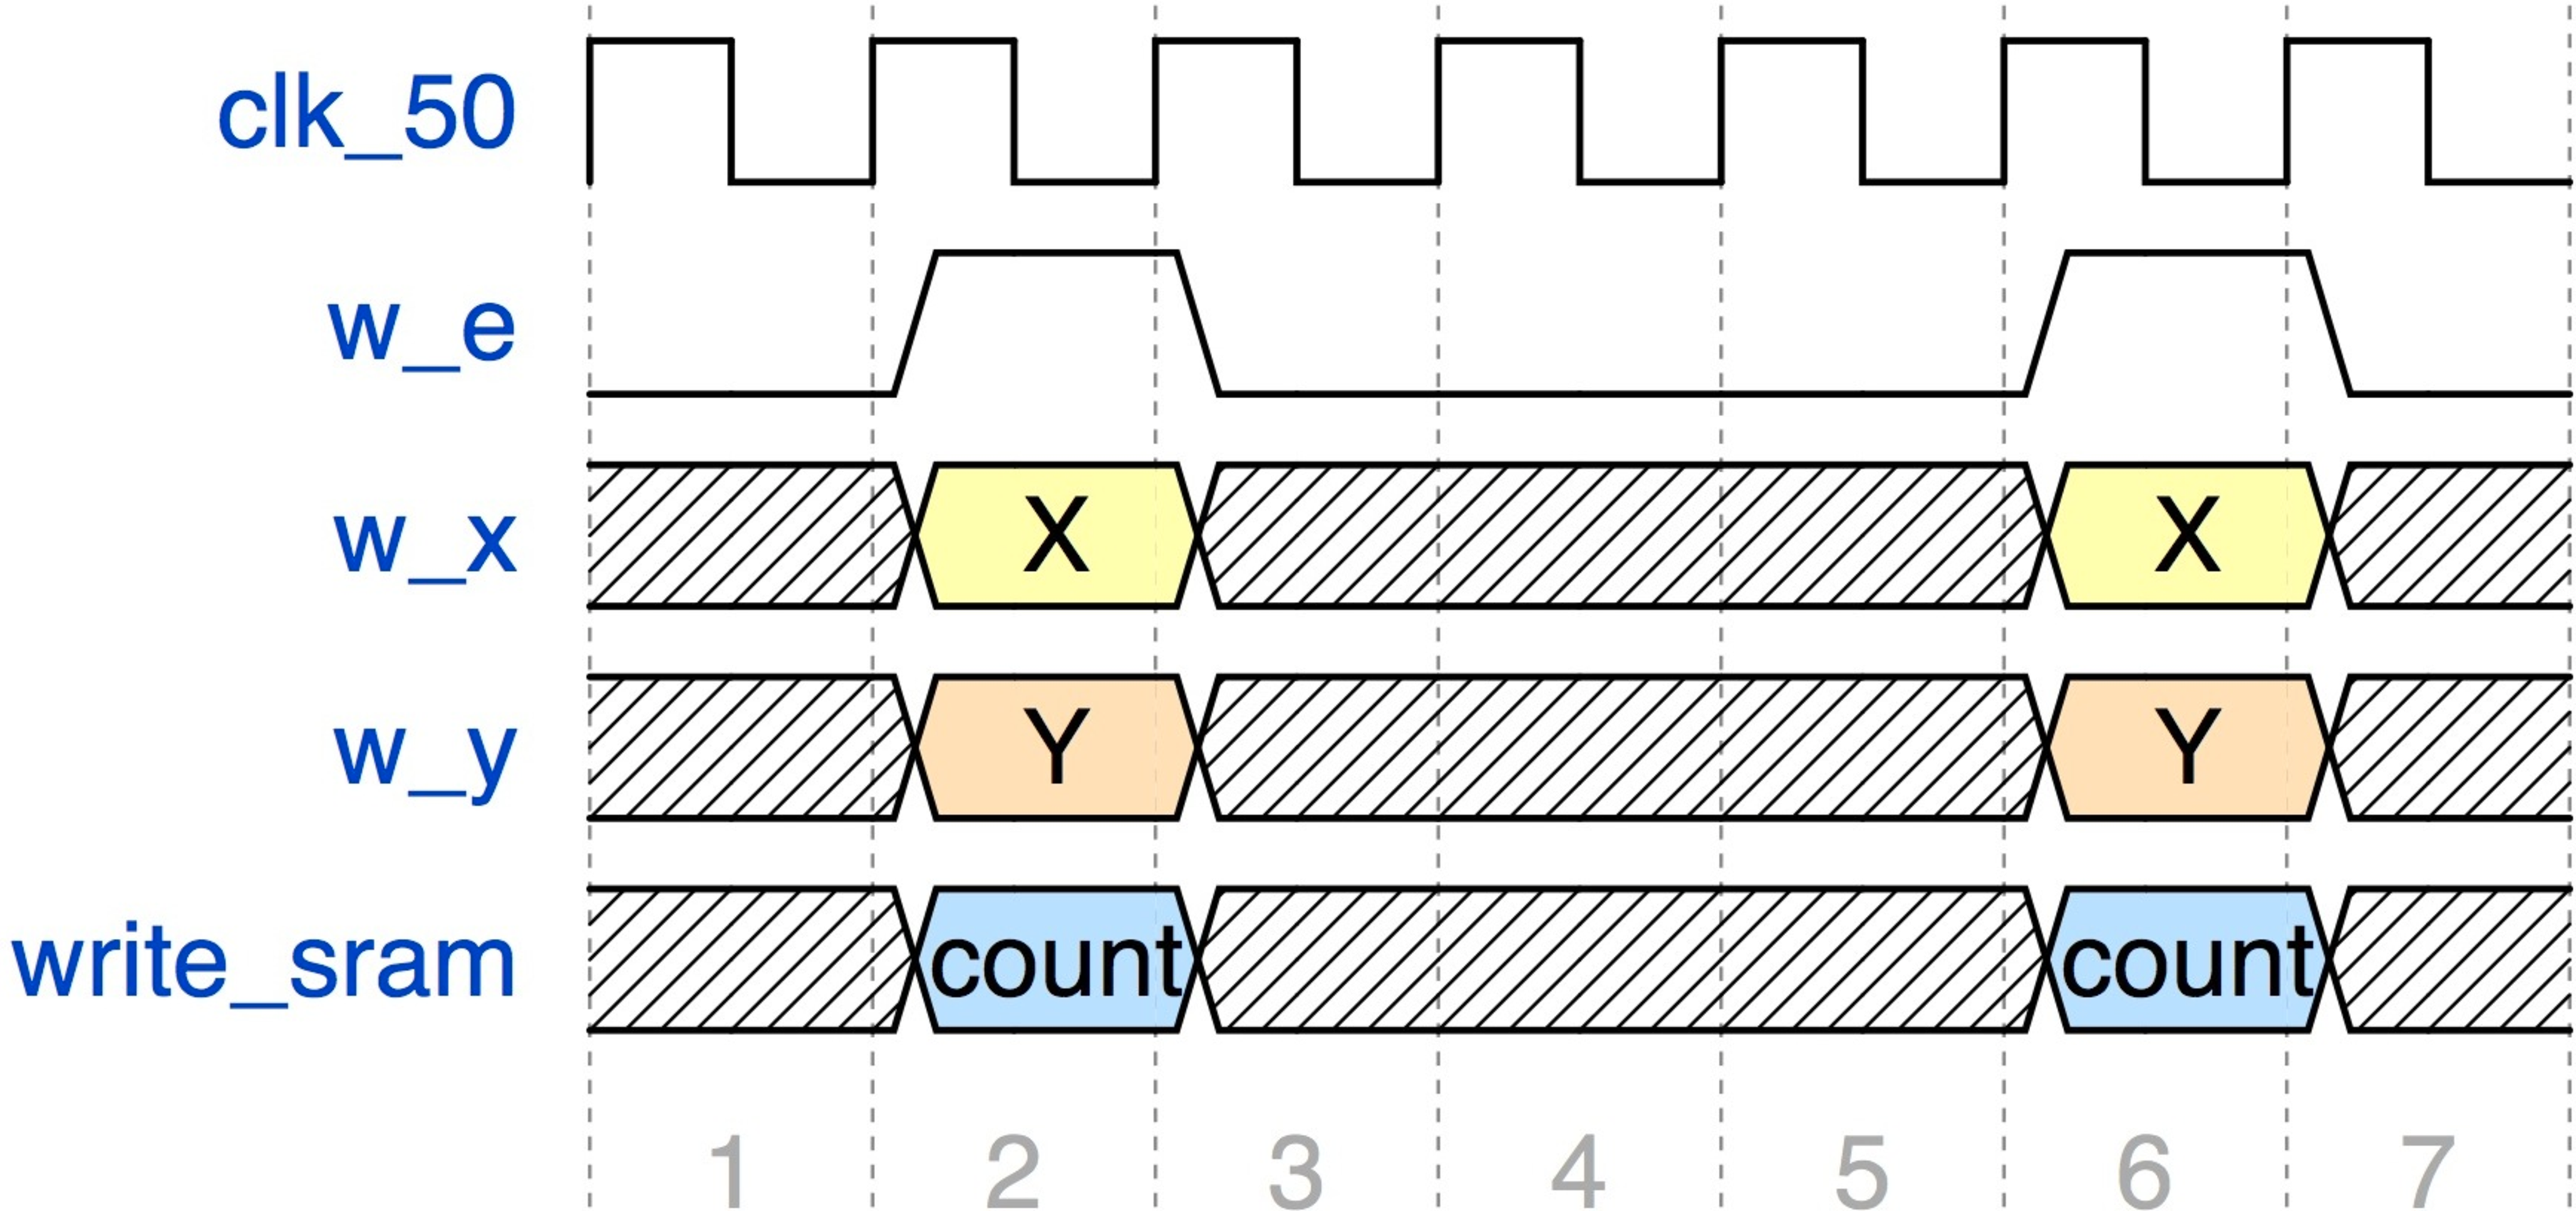
\includegraphics[width=300pt]{timing_diagrams/ifm_clut.pdf}
  \caption{Timing diagram of the interface between the \texttt{IFM}s and the \texttt{Coordinate-Breakaway LUT}.}
\end{figure}


\subsubsection{VGA Module}

In order to display the generated Julia set, we connect a VGA controller 
 to the \texttt{Coordinate-Breakaway lookup table}. As the controller cycles
through output coordinates within the display area, it modifies the
read address signal for the lookup table. The data signal coming from
the RAM is thus the breakaway value associated with that coordinate.

\begin{figure}[H]
  \centering
    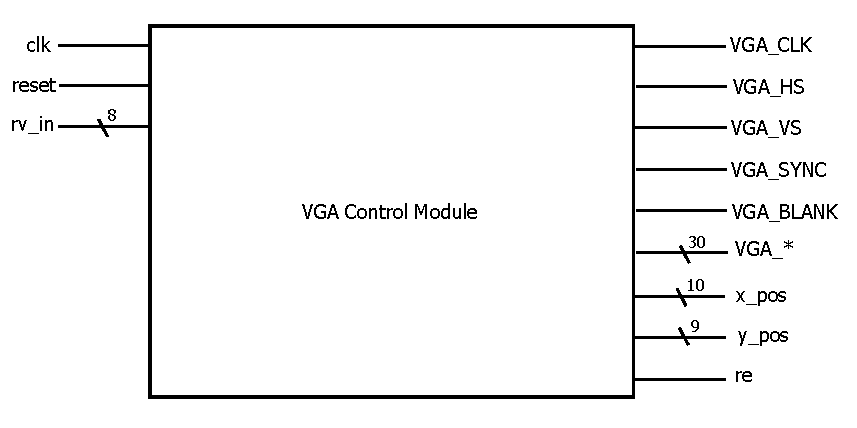
\includegraphics[width=300pt]{block_diagrams/vga.pdf}
  \caption{Block diagram of the VGA module}
\end{figure}

This breakaway value is passed through a decoder known as the
\texttt{Colorization lookup table} and the resulting $(R, G, B)$ signal tuple
is sent to the VGA port.

\subsubsection{Colorization lookup table}
The \texttt{Colorization lookup table} is implemented using a ROM on the FPGA. The ROM maps each possible breakaway $k$ value to a bit-vector corresponding to the $(R, G, B)$ signal tuple that should be expressed for that value.
The system includes a special ``cycle colors'' mode, wherein the $k$ value being sent in to the \texttt{Colorization 
lookup table} is modified by a linearly increasing amount. This causes the colors to shift on screen, creating a 
remarkable aesthetic.

To assist with programming the ROM, the development team created a small Python application that allows the user
to graphically modify $(R, G, B)$ components for different $k$ values, and interpolates the results. The application 
can then display a preview of what a Julia set will look like with these settings, and produces VHDL for programming
the ROM accordingly.

% ----------------------------------------
% figures for the VGA


\begin{figure}
  \centering
    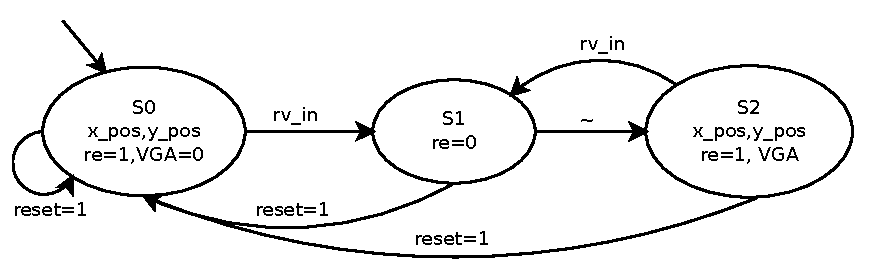
\includegraphics[width=200px]{state_diagrams/vga.pdf}
  \caption{State diagram for the \texttt{VGA module}, Mealy machine: $\thicksim$
    stands in for no input/output, and VGA stands in for all the \texttt{VGA\_}
    signals (\texttt{VGA\_CLK}, \texttt{VGA\_HS}, \texttt{VGA\_VS},
    \texttt{VGA\_BLANK}, \texttt{VGA\_SYNC}, \texttt{VGA\_R}, \texttt{VGA\_G},
    \texttt{VGA\_B}). Omits unused signals for compactness.}
\end{figure}


% ------------------------------------------------------------

%These modules might be used parameterize the output fractal

%\begin{itemize}
%\item PS/2 Keyboard input can be used to allow the user to specify
%  fractal recomputation using a different set of parameters,
%  permitting the modification of window ranges and Julia set
%  constants. Keyboard input would be facilitated through the Nios II
%  processor and would require a reexecution of the Window Generator.
%\item We could create a module for permuting the display colors given
%  by the Colorization Lookup table using a periodic function, thus
%  causing the colors to cycle. This module would allow us to modify
%  the way the fractal looks without recomputing it.
%\end{itemize}

\section{System Validation and Performance}

\subsection{Verification and Validation}

During development of the Interactive Fractal Viewer, it was desireable to validate the functionality of
individual components. We used VHDL Test Benches in combination with the Quartus RTL simulation tool to verify proper timing and behavior during the early stages of development.

The development team wrote Test Benches for each of the major hardware components. These proved invaluable in 
finding problems during the initial implementation stages, as well as diagnosing them later on. 

Additionally, in order to strictly verify the correctness of the Julia sets that the system produced, the team wrote a 
specialized Test Bench capable of dumping $(a, b, k)$  triples to a file. A Python
script was written to parse and validate this file. The script built a complex number for each $(a, b)$ double 
and computed its own breakaway iteration $k'$ for that value using floating point precision. If the $|k-k'|<\epsilon$, 
it marks the value as a success. Otherwise, it is marked as a failure. The tolerance parameter $\epsilon$ is necessary
because Julia set iterations represent chaotic systems. Therefore, the minor perturbations caused by the difference
in hardware vs. software computation can cause major changes.

For the Julia set described by a chosen $c$, and $\epsilon = 5$, the validation script showed a $98$\% success rate on
the $307200$ points tested.

\subsection{Performance Analysis}

\subsubsection{Upper-Bound on Image Generation Time}

Say the system wishes to compute an arbitrary window of an arbitrary Julia set. The only variable in generation time for a given
image is the amount of time it takes for the \texttt{IFM}s to completely write all $k$ values to the \texttt{Coordinate-Breakaway lookup table}. Thus, to find an upper bound on image generation time, we may assume that
each \texttt{IFM} spends the maximum possible amount of time computing the $k$ value for each coordinate. The 
number of iterations in each \texttt{IFM} is capped at $127$. Each \texttt{IFV} can perform one function evaluation
per clock cycle, and requires $3$ cycles of setup and tear-down time for state changes. 

Additionally the \texttt{IFM Controller} takes a clock cycle between each \texttt{IFM} value assignment to perform a check for a ready \texttt{IFM} and grab a new value from the \texttt{Window Generator}. 

Thus, the system sets up a pipeline extending from the \texttt{IFV Controller} to the \texttt{Coordinate-Breakaway lookup table}. When using $4$ \texttt{IFM}s for computation, it may achieve a throughput of $\frac{4\; \text{values}}{133\; \text{iterations}}$ 

Though the system has to worry about
scheduling conflicts from the controller on the first set of values to go to the \texttt{IFM}s (since only one \texttt{IFM} may be assigned or report a value at a once), this issue vanishes due to pipelining on subsequent value sets because maximizing the number of iterations required for each value means synchronizing the start and end times of each \texttt{IFM}.

It is now possible compute the delay incurred between the \texttt{IFM Controller} and the \texttt{Coordinate-Breakaway lookup table} when generating a full image on a 25MHz clock in this scenario. $640 \times 480 = 307200$ values must be computed, so

$$
\frac{307200\; \text{values}}{1\; \text{image}} \times \frac{133 \;\text{iterations}}{4 \;\text{values}} \times \frac{1 \;\text{cycle}}{1 \;\text{iteration}} \times \frac{1 \;\text{seconds}}{25000000 \;\text{cycles}} = \frac{0.408576 \;\text{seconds}}{\text{image}}
$$

Which is a good approximation of the upper bound on total time it takes for data to flow through the system.

\subsubsection{Experimental Results}

Simulations on a variety of constants confirmed the above results, producing delays ranging from $0.125s$ to $0.250s$ 
on use case images, and a delay of $0.409s$ on a ``maximum cost'' image. 

\section{Milestone Report}

\begin{tabular}{rlp{4.5cm}p{4.5cm}}
\textbf{Milestone}&\textbf{Date}&\textbf{Goal}&\textbf{Accomplished}\\ \hline
&&&\\
Milestone 1&Mar 27&Have a static Julia set filled into a buffer.&
	Develop a \texttt{Window Generator} capable of communicating with a parallelized \texttt{IFM Controller}\\
&&&\\
Milestone 2&Apr 10&Display the colorized Julia set through VGA.&\textit{As planned.}\\
&&&\\
Milestone 3&Apr 24&Implement parameter mutation, with subsequent updates to the displayed Julia set.&
	Hardware-based parameter mutation and set redraw.\\
&&&\\
Deadline&May 9&Feature-complete system with accompanying report and presentation.&\textit{As planned.}\\
&&&\\
\end{tabular}

\section{Contributions and Teamwork}

As in all good engineering projects, our development team was heavily collaborative. There are very few
files in our source that were produced by one person alone. However, our modular development process allowed
different team members to accept primary responsibility for certain files. The following is a list of major
contributions of each team member to the project 

\begin{itemize}

\item
\textbf{Nathan Hwang}
\begin{enumerate}
\item Project management work
\item \texttt{Coordinate-Breakaway lookup table}
\item VHDL for color cycling
\item Instruction registers for communication with NIOS
\end{enumerate}

\item 
\textbf{Richard Nwaobasi}
\begin{enumerate}
\item \texttt{Colorization lookup table}
\item \texttt{VGA Module}
\item Communication with PS/2 keyboard
\item Control loop software (with Stephen Pratt)
\end{enumerate}

\item 
\textbf{Luis Pe\~{n}a}
\begin{enumerate}
\item Systems integration
\item Top level module
\item \texttt{IFM} and \texttt{IFM Controller}
\item Parameterization RAM (with Stephen Pratt)
\end{enumerate}

\item 
\textbf{Stephen Pratt}
\begin{enumerate}
\item Document composition and presentaiton management
\item Integration test bench and validation script
\item \texttt{Window Generator} and window generation algorithm
\item Parameterization RAM (with Luis Pe\~{n}a)
\item Control loop software (with Richard Nwaobasi)
\end{enumerate}

\end{itemize}


\section{Challenges and Lessons Learned}

This project was one filled with learning opportunities, both in terms of technical knowlege as well as
personal growth. Some major design and implementation challenges included:

\begin{enumerate}{}
\item \textbf{Design and Implementation of the IFMs} - Working with a system as parallel and dynamic as our \texttt{IFM} array presented a very unique set of challenges. Many communication protocols, state machines, and design concepts were
discussed when planning the design of this core component of our device. Because most elements of our system needed
to interface with the \texttt{IFM Controller} in some way, successful integration of the component was in many ways a cornerstone acheivement for our team.

\item \textbf{Maintaining Timing Discipline} - Clocks were consistently an adversary for our team, as many parts 
of our system needed to operate at different rates. The NIOS processor and the buses it writes to necessarily run at 50MHz, while the critical path on our \texttt{IFM}s allowed for only 25MHz frequencies. The SDRAM clock needed to lag the NIOS to account for setup, charging, and hold times, and the VGA clock needed to run at just over 25MHz to meet protocol. We did run into trouble on many occasions when trying to manage interplay between these components, but this taught us a lot about the importance of synchronization in Embedded Systems and the nature of Phase-Locked Loops.

\end{enumerate}

Furthermore, each group member ended up with a few personal takeaways:

\begin{itemize}

\item
\textbf{Nathan Hwang}
\begin{enumerate}
\item Between the team and the tools, the team is the greater.
\end{enumerate}

\item 
\textbf{Richard Nwaobasi}
\begin{enumerate}
\item I would say that while it's good to enjoy early success, keep in mind that the the road to a project's final realization is a long and uneven one. In addition to this, form good relationships with your teammates: it makes those late nights that turn into early mornings all the more bearable, and at times even enjoyable and worthwhile.
\end{enumerate}

\item 
\textbf{Luis Pe\~{n}a}
\begin{enumerate}
\item Modularity is golden. The team divided up the IFV into smaller components to be able to test their functions easily. This modularity helped so much that the first time we connected the core components, they all worked.
\item Meeting with the team early on to discuss interfaces and protocols was really useful because we did not have to work together all the time to create our individual components.
\item We should have listened more to Dr. Edwards because he knows about many of the issues we faced. We should have made more use of his office hours, especially because he was our adviser for the project. 
\end{enumerate}

\item 
\textbf{Stephen Pratt}
\begin{enumerate}
\item Consistent progress is of central importance to the success of a project. A team should always focus on 
moving forward at least a little bit, no matter how busy the week. Even the most marginal rates of progress are far preferable
to the overhead that ends up getting poured into teardown/setup time if a team decides to focus its efforts elsewhere
for even a short period.
\item Implementation challenges are not exam questions. They do not need to be solved alone, or even successfully on 
the first go around. It's far better to experiment and utilize resources that are available than to design a failing
solution and pour time into trying to make the implementation work out.
\end{enumerate}

\end{itemize}


\section{Reflections and Prospective}

All things considered, our team is extremely satisfied with the results that we've achieved. 
Development was certainly not without its ups and downs, but we ultimately brought all major project
goals to fruition. 

Of course, like all good engineers, we can never claim to be completely satisfied with the fruits of our
labor. The following are a few features that we would like to implement once we have more time 
to work with the project:

\begin{enumerate}
\item Though window and constant selection are currently software-mutable system parameters, the UI through
which these parameters are modified does not allow very intuitive control of their values. A primary reason
for this is that our original system architecture was built with the explicit purpose of drawing fractals on the
screen, not anything else. In the future, we would like to let users select a custom window by modifying a frame 
on-screen. Explicit, rather than relative specification of new seed constants for the Julia set would also be 
desirable.
\item There exist a few timing glitches that were never completely resolved. Ironing out these glitches is a high
priority for future work.
\item It is our professional opinion that the color-cycle mode is totally radical. Having this cycling rate vary 
with audio input would turn our Interactive Fractal Viewer into a spectacular music visualizer.
\end{enumerate}

\appendix
\section{Source Code}
\subsection{VHDL}
\subsubsection{ifv.vhd}							%All

\begin{lstlisting}
--------------------------------------------------------------------
-- DE2 top-level module for the IFV
--
-- Nathan Hwang, Richard Nwaobasi, Luis E. P. & Stephen Pratt
--
-- From an original by Terasic Technology, Inc.
-- (DE2_TOP.v, part of the DE2 system board CD supplied by Altera)
--------------------------------------------------------------------
library ieee;
use ieee.std_logic_1164.all;
use ieee.numeric_std.all;

entity ifv is

	port (
	CLOCK_50	: in std_logic;                    -- 50 MHz

	-- LED displays
	HEX0, HEX1, HEX2, HEX3, HEX4, HEX5, HEX6, HEX7 -- 7-segment displays
	: out std_logic_vector(6 downto 0);
	LEDG : out std_logic_vector(8 downto 0);       -- Green LEDs

	-- SDRAM
	DRAM_DQ : inout std_logic_vector(15 downto 0); -- Data Bus
	DRAM_ADDR : out std_logic_vector(11 downto 0); -- Address Bus    
	DRAM_LDQM,                                     -- Low-byte Data Mask 
	DRAM_UDQM,                                     -- High-byte Data Mask
	DRAM_WE_N,                                     -- Write Enable
	DRAM_CAS_N,                                    -- Column Address Strobe
	DRAM_RAS_N,                                    -- Row Address Strobe
	DRAM_CS_N,                                     -- Chip Select
	DRAM_BA_0,                                     -- Bank Address 0
	DRAM_BA_1,                                     -- Bank Address 0
	DRAM_CLK,                                      -- Clock
	DRAM_CKE : out std_logic;                      -- Clock Enable

	-- SRAM   
	SRAM_DQ : inout std_logic_vector(15 downto 0); -- Data bus 16 Bits
	SRAM_ADDR : out std_logic_vector(17 downto 0); -- Address bus 18 Bits
	SRAM_UB_N,                                     -- High-byte Data Mask 
	SRAM_LB_N,                                     -- Low-byte Data Mask 
	SRAM_WE_N,                                     -- Write Enable
	SRAM_CE_N,                                     -- Chip Enable
	SRAM_OE_N : out std_logic;                     -- Output Enable	

	-- PS/2 port
	PS2_DAT,                    -- Data
	PS2_CLK : inout std_logic;     -- Clock

	-- VGA output
	VGA_CLK,                                            -- Clock
	VGA_HS,                                             -- H_SYNC
	VGA_VS,                                             -- V_SYNC
	VGA_BLANK,                                          -- BLANK
	VGA_SYNC : out std_logic;                           -- SYNC
	VGA_R,                                              -- Red[9:0]
	VGA_G,                                              -- Green[9:0]
	VGA_B : out unsigned(9 downto 0)                   -- Blue[9:0]
);
  
end ifv;

architecture datapath of ifv is

	signal clk_25			: std_logic;
	signal clk_50			: std_logic;
	signal clk_sdram		: std_logic;

	signal cread			: unsigned(7 downto 0);
	signal xread			: unsigned(9 downto 0);
	signal yread			: unsigned(8 downto 0);
	signal re				: std_logic;
	signal we				: std_logic;
	signal cwrite			: unsigned(7 downto 0);
	signal xwrite			: unsigned(9 downto 0);
	signal ywrite			: unsigned(8 downto 0);

	signal a_min			: signed(35 downto 0)		:= X"F80000000";
	signal b_min			: signed(35 downto 0)		:= X"FA0000000";
	signal a_diff			: signed(35 downto 0)		:= X"000666666";
	signal b_diff			: signed(35 downto 0)		:= X"000666666";
	signal cr   			: signed(35 downto 0)		:= X"FCA8F5C29";
	signal ci   			: signed(35 downto 0)		:= X"FF125460B";
	signal a_leap			: unsigned(9 downto 0)		:= "0000000010";
	signal b_leap			: unsigned(9 downto 0)		:= "0000000010";
	signal reset_n			: std_logic							:='1';

	signal a_mine			: signed(35 downto 0)		;
	signal b_mine			: signed(35 downto 0)		;
	signal a_diffe			: signed(35 downto 0)		;
	signal b_diffe			: signed(35 downto 0)		;
	signal cre   			: signed(35 downto 0)		;
	signal cie   			: signed(35 downto 0)		;
	signal a_leape			: unsigned(9 downto 0)		;
	signal b_leape			: unsigned(9 downto 0)		;

	signal DRAM_BA			: std_logic_vector(1 downto 0);
	signal DRAM_DQM			: std_logic_vector(1 downto 0);

	signal ram_read			: std_logic;
	signal ram_data			: signed(17 downto 0);
	signal ram_address		: unsigned(3 downto 0);
	signal ram_addr			: unsigned(3 downto 0);

	signal iterate			: std_logic;
	signal reset			: std_logic;
	signal color			: std_logic_vector(2 downto 0);
	signal refresh			: std_logic;
	signal fract			: std_logic_vector(1 downto 0);
	signal sig				: std_logic_vector(7 downto 0);
	begin

	reset					<= sig(0);
	iterate					<= sig(1);
	color					<= sig(4 downto 2);
	refresh					<= sig(5);
	fract					<= sig(7 downto 6);
	LEDG(7 downto 0)		<= sig;

	process (clk_25)
	begin
		if rising_edge(clk_25) then

			if fract = "00" then
				a_min		<= a_mine;
				b_min		<= b_mine;
				a_diff		<= a_diffe;
				b_diff		<= b_diffe;
				cr			<= cre;
				ci			<= cie;
				a_leap		<= a_leape;
				b_leap		<= b_leape;
			elsif fract = "01" then
				a_min		<= X"F80000000";
				b_min		<= X"FA0000000";
				a_diff		<= X"000666666";
				b_diff		<= X"000666666";
				cr			<= X"000000000";
				ci			<= X"000000000";
				a_leap		<= "0000000010";
				b_leap		<= "0000000010";
			elsif fract = "10" then
				a_min		<= X"F80000000";
				b_min		<= X"FA0000000";
				a_diff		<= X"000666666";
				b_diff		<= X"000666666";
				cr			<= X"FCA8F5C29";
				ci			<= X"FF125460B";
				a_leap		<= "0000000010";
				b_leap		<= "0000000010";
			else
				a_min		<= X"F80000000";
				b_min		<= X"FA0000000";
				a_diff		<= X"000666666";
				b_diff		<= X"000666666";
				cr			<= X"FCA8F5C29";
				ci			<= X"FFF25460B";
				a_leap		<= "0000000010";
				b_leap		<= "0000000010";
			end if;
		end if;
	end process;

	VGA_CLK   <= clk_25;
	DRAM_BA_1 <= DRAM_BA(1);
	DRAM_BA_0 <= DRAM_BA(0);
	DRAM_UDQM <= DRAM_DQM(1);
	DRAM_LDQM <= DRAM_DQM(0);
	DRAM_CLK  <= clk_sdram;

CLK5025: entity work.pll5025 port map(
	inclk0	=> CLOCK_50,
	c0		=> clk_50,
	c1		=> clk_25,
	c2		=> clk_sdram
	);

IFM: entity work.hook port map(
	clk25		=> clk_25,
	reset		=> reset,
	a_min		=> a_min,
	a_diff		=> a_diff,
	a_leap		=> a_leap,
	b_min		=> b_min,
	b_diff		=> b_diff,
	b_leap		=> b_leap,
	cr			=> cr,
	ci			=> ci,
	std_logic_vector(xout)		=> xwrite,
	std_logic_vector(yout)		=> ywrite,
	count		=> cwrite,
	we			=> we
	);

NIOS: entity work.nios port map (
 -- 1) global signals:
	clk								=> clk_50,
	clk_25							=> clk_25,
	reset_n							=> '1',

	PS2_CLK_to_and_from_the_ps2_0	=> PS2_CLK,
	PS2_DAT_to_and_from_the_ps2_0	=> PS2_DAT,
	irq_from_the_ps2_0				=> LEDG(8),

 -- the_ram
	addressout_to_the_ram			=> std_logic_vector(ram_address),
	read_to_the_ram					=> ram_read,
	std_logic_vector(readdata_from_the_ram)		=> ram_data,
	std_logic_vector(readaddr_from_the_ram)		=> ram_addr,
	
 -- the sram signal
	read_addr_to_the_ram_signal		=> '0',
	read_data_from_the_ram_signal 	=> sig,

 -- the_sdram
	zs_addr_from_the_sdram		=> DRAM_ADDR,
	zs_ba_from_the_sdram		=> DRAM_BA,
	zs_cas_n_from_the_sdram		=> DRAM_CAS_N,
	zs_cke_from_the_sdram		=> DRAM_CKE,
	zs_cs_n_from_the_sdram		=> DRAM_CS_N,
	zs_dq_to_and_from_the_sdram	=> DRAM_DQ,
	zs_dqm_from_the_sdram		=> DRAM_DQM,
	zs_ras_n_from_the_sdram		=> DRAM_RAS_N,
	zs_we_n_from_the_sdram		=> DRAM_WE_N
 );

RMR: entity work.rammer port map(
	clk				=> clk_25,
	compute			=> refresh,
	read			=> ram_read,
	addressout		=> ram_address,
	addressin		=> ram_addr,
	readdata		=> ram_data,
	amin			=> a_mine,
	bmin			=> b_mine,
	adiff			=> a_diffe,
	bdiff			=> b_diffe,
	aleap			=> a_leape,
	bleap			=> b_leape,
	cro				=> cre,
	cio				=> cie
	);

VGA: entity work.vga_mod port map (
	clk			=> clk_25,
	reset		=> '0',
	switch		=> color,
	count		=> cread,--EXTERNAL SIGNALS
	VGA_HS		=> VGA_HS,
	VGA_VS		=> VGA_VS,
	VGA_BLANK	=> VGA_BLANK,
	VGA_SYNC	=> VGA_SYNC,
	VGA_R		=> VGA_R,
	VGA_G		=> VGA_G,
	VGA_B		=> VGA_B,
	xout		=> xread,--EXTERNAL SIGNALS
	yout		=> yread,--EXTERNAL SIGNALS
	re  		=> re,--EXTERNAL SIGNALS
	ce  		=> iterate
	);

SRAM: entity work.sram port map(
	sram_data	=> SRAM_DQ,
	sram_addr	=> SRAM_ADDR,
	sram_ub_n	=> SRAM_UB_N,
	sram_lb_n	=> SRAM_LB_N,
	sram_we_n	=> SRAM_WE_N,
	sram_ce_n	=> SRAM_CE_N,
	sram_oe_n	=> SRAM_OE_N,
	rx			=> std_logic_vector(xread),
	ry			=> std_logic_vector(yread),
	wx			=> std_logic_vector(xwrite),
	wy			=> std_logic_vector(ywrite),
	std_logic_vector(rv)	=> cread,
	wv			=> std_logic_vector(cwrite),
	re			=> re,
	we			=> we
	);
  
	HEX7     <= "1100001"; -- J
	HEX6     <= "1000001"; -- U
	HEX5     <= "1000111"; -- L
	HEX4     <= "1111001"; -- I
	HEX3     <= "0001000"; -- A
	HEX2     <= "0010010"; -- S
	HEX1     <= "0000110"; -- E
	HEX0     <= "0000111"; -- t
end datapath;
\end{lstlisting}

\subsubsection{ramcon.vhd}							%Luis
\begin{lstlisting}
---------------------------------------------------------------------
--ramcon
--
--This is the entity holding all four IFMs. This is where all the
--wiring and the IFM coordination takes place.
--
--Author: Luis E. P.
---------------------------------------------------------------------
library ieee;
use ieee.std_logic_1164.all;
use ieee.numeric_std.all;

entity ramcon is
	port(
	clk						: in std_logic;
	reset_n					: in std_logic;
	read					: in std_logic;
	write					: in std_logic;
	chipselect				: in std_logic;
	address					: in unsigned(3 downto 0);
	addressout				: in unsigned(3 downto 0);
	
	readaddr				: out unsigned(3 downto 0);
	readdata				: out unsigned(17 downto 0);
	writedata				: in unsigned(31 downto 0)
	);
end ramcon;

architecture ramarch of ramcon is

	type ram_type is array(15 downto 0) of unsigned(17 downto 0);
	signal RAM				: ram_type;
	begin

	process(clk)
	begin
		if rising_edge(clk) then
			readaddr	<= addressout;
			readdata	<= RAM(to_integer(addressout));
			if chipselect = '1' then
				if write = '1' then
					RAM(to_integer(address))	<= writedata(17 downto 0);
				end if;
			end if;
		end if;
	end process;
	
	
end ramarch;
\end{lstlisting}
\subsubsection{rammer.vhd}							%Luis


\subsubsection{window\_gen.vhd}					%Steve	

\begin{lstlisting}
---------------------------------------------------------------------
--window_gen.vhd
--
--A device used to generate (a, b) values for each pixel on the
--screen under the given window parameters.
--
--Author: Stephen Pratt
---------------------------------------------------------------------


library ieee;
use ieee.std_logic_1164.all;
use ieee.numeric_std.all;

entity window_gen is
  
  port (
    clk        	: in std_logic;
	next_val	: in std_logic;
	reset		: in std_logic;
    
	a_min		: in signed(35 downto 0);
	a_diff		: in signed(35 downto 0);
	a_leap		: in unsigned(9 downto 0);
	b_min		: in signed(35 downto 0);
	b_diff		: in signed(35 downto 0);
	b_leap		: in unsigned(9 downto 0);
	
	a_out		: out std_logic_vector(35 downto 0);
	b_out		: out std_logic_vector(35 downto 0);
	x_out		: out std_logic_vector(9 downto 0);
	y_out		: out std_logic_vector(9 downto 0);
	ready		: out std_logic
	);
  
end window_gen;

architecture wg of window_gen is 

constant HACTIVE	: integer := 640-1;
constant VACTIVE	: integer := 480-1;

signal x_max 		: unsigned(9 downto 0) := to_unsigned(HACTIVE, 10);
signal y_max 		: unsigned(9 downto 0) := to_unsigned(VACTIVE, 10);

signal a_at_max		: std_logic;
signal b_at_max		: std_logic;
signal both_max		: std_logic;

signal a_ready		: std_logic;
signal b_ready		: std_logic;

signal b_next		: std_logic;
signal a_reset		: std_logic;

signal y_out_mirror	: std_logic_vector(9 downto 0);

begin

	b_next <= next_val and a_at_max;
	
	both_max <= a_at_max and b_at_max;
	
	a_reset <= reset or (b_next and not both_max); 
	y_out <= std_logic_vector(y_max - unsigned(y_out_mirror));
	
	ready <= a_ready and b_ready;

	--Module is composed of two diff_counters, one for each
	--screen dimension.
	a_counter:	entity work.diff_counter port map (
		clk 		=> clk,
		next_val 	=> next_val,
		reset 		=> a_reset,		
		
		v_min 		=> a_min,
		v_diff		=> a_diff,
		v_leap		=> a_leap,
		max_itr		=> x_max,
		
		v_out		=> a_out,
		c_out		=> x_out,
		at_max		=> a_at_max,
		ready		=> a_ready
	);
	
	
	b_counter:	entity work.diff_counter port map (
		clk 		=> clk,
		next_val 	=> b_next,
		reset 		=> reset,		
		
		v_min 		=> b_min,
		v_diff		=> b_diff,
		v_leap		=> b_leap,
		max_itr		=> y_max,
		
		v_out		=> b_out,
		c_out		=> y_out_mirror,
		at_max		=> b_at_max,
		ready		=> b_ready
	);	

end wg;
\end{lstlisting}

\subsubsection{diff\_counter.vhd}					%Steve


\begin{lstlisting}
---------------------------------------------------------------------
--diff_counter.vhd
--
--A device that increments a value by some differential, adjusting 
--the sum as necessary to assure convergence to a maximum value.
--
--Author: Stephen Pratt
---------------------------------------------------------------------

library ieee;
use ieee.std_logic_1164.all;
use ieee.numeric_std.all;

entity diff_counter is
  
  port (
    clk        	: in std_logic;
	next_val	: in std_logic;
	reset		: in std_logic;
    
	v_min		: in signed(35 downto 0);
	v_diff		: in signed(35 downto 0);
	v_leap		: in unsigned(9 downto 0);
	max_itr		: in unsigned(9 downto 0);
	
	v_out		: out std_logic_vector(35 downto 0);
	c_out		: out std_logic_vector(9 downto 0);
	at_max		: out std_logic;
	ready		: out std_logic
    );
  
end diff_counter;

architecture dc of diff_counter is 

signal itr_count 	: unsigned (9 downto 0);
signal leap			: std_logic;
signal v_next		: signed(35 downto 0);
signal c_next		: unsigned(9 downto 0);
signal itr_next		: unsigned(9 downto 0);
signal v_curr		: signed(35 downto 0);
signal c_curr		: unsigned(9 downto 0);

signal v_sum		: signed (35 downto 0);
signal ready_sig 	: std_logic := '0';

begin

c_out <= std_logic_vector(c_curr);
v_out <= std_logic_vector(v_curr);
ready <= ready_sig;

process(clk)

begin	

	if rising_edge(clk) then

		c_next <= c_curr+1;
		v_next <= v_curr + v_diff;
		
		itr_next <= itr_count+1; --itr_next is leap counter
		
		--make adjustment on leap count
		if leap = '1' then 
			v_next <= v_curr + v_diff + 1;
			itr_next <= (others=>'0'); --reset leap counter to zero
		end if;

		leap <= '0';
		
		--if we complete a leap interval, we should leap next cycle
		if itr_next = v_leap then
			leap <= '1';
		end if;	

		itr_count <= itr_count;		
		
		--Reset operation - tra---------------------------------------------------------------------
--vga_mod.vhd
--
--This unit connects the VGA raster and the Color_LUT.
--
--Author: Richard Nwaobasi
---------------------------------------------------------------------

library ieee;
use ieee.std_logic_1164.all;
use ieee.numeric_std.all;

entity vga_mod is
	port(
		clk, reset	: in std_logic;
		count		: in unsigned(7 downto 0);
		switch		: in std_logic_vector(2 downto 0);
		VGA_HS,                                 -- H_SYNC
		VGA_VS,                                 -- V_SYNC
		VGA_BLANK,                              -- BLANK
		VGA_SYNC	: out std_logic;            -- SYNC
		VGA_R,                                  -- Red[9:0]
		VGA_G,                                  -- Green[9:0]
		VGA_B		: out unsigned(9 downto 0); -- Blue[9:0]
		xout		: out unsigned(9 downto 0);
		yout		: out unsigned(8 downto 0);
		re  		: out std_logic;
		ce  		: in std_logic
	);
end vga_mod;

architecture imp of vga_mod is

  component vga
    port (
    reset   : in std_logic;
    clk     : in std_logic;                    -- Should be 25.125 MHz
    VGA_RGB : in unsigned(29 downto 0);
    VGA_HS,                           -- H_SYNC
    VGA_VS,                           -- V_SYNC
    VGA_BLANK,                        -- BLANK
    VGA_SYNC : out std_logic;         -- SYNC
    VGA_R,                            -- Red[9:0]
    VGA_G,                            -- Green[9:0]
    VGA_B : out unsigned(9 downto 0); -- Blue[9:0]
    x_pos : out unsigned(9 downto 0);
    y_pos : out unsigned(8 downto 0);
    re    : out std_logic             -- Read Enable
		);
  end component;
	
  component Color_LUT
    port(
      count   : in unsigned(7 downto 0);
      switch  : in std_logic_vector(2 downto 0);
      VGA_RGB : out unsigned(29 downto 0));
  end component;

	signal VGA_RGB    : unsigned(29 downto 0);

	signal cycle : unsigned(7 downto 0) := (others => '0');
	signal spacer : unsigned(19 downto 0) := (others => '0');

begin
  
  G : vga port map (reset => reset,
					clk => clk,                -- Should be 25.125 MHz
					VGA_RGB => VGA_RGB,
					VGA_HS     => VGA_HS,
					VGA_VS     => VGA_VS,
					VGA_BLANK  => VGA_BLANK,
					VGA_SYNC   => VGA_SYNC,
					VGA_R      => VGA_R,
					VGA_G      => VGA_G,
					VGA_B      => VGA_B,
					x_pos	  => xout,
					y_pos	  => yout,
					re		  => re);

   A : Color_LUT port map 
		(count		=> count + cycle,
		switch		=> switch,
		VGA_RGB		=> VGA_RGB);

	process(clk)
	begin
		if rising_edge(clk) then
			if reset = '1' then
				spacer <= (others => '0');
				cycle <= (others => '0');
			end if;
			if ce = '1' then
				spacer <= spacer + 1;
				if spacer = 0 then
					cycle <= cycle + 1;
				end if;
			end if;
		end if;
	end process;

end imp;nsition to start state
		if reset = '1' then
			v_curr <= v_min;
			c_curr <= (others=>'0');
			itr_count <= (others=>'0');
			at_max <= '0';
			ready_sig <= '1';
			
		--Maximum iteration reached - transition to max state
		elsif c_curr = max_itr then
			at_max <= '1';
			
		--Next value requested
		elsif next_val = '1' then			
			c_curr <= c_next;
			v_curr <= v_next;			
			itr_count <= itr_next;					
		end if;
		
	end if;
end process;

end dc;
\end{lstlisting}

\subsubsection{hook.vhd}							%Luis


\begin{lstlisting}
---------------------------------------------------------------------
--hook.vhd
--
--This is the place where the IFMs and their controller connect with
--the window generator that feeds the IFMs.
--
--Author: Luis E. P.
---------------------------------------------------------------------
library ieee;
use ieee.std_logic_1164.all;
use ieee.numeric_std.all;

entity hook is
	port(
	clk25		: in std_logic;
	reset		: in std_logic;								-- Clear
	a_min		: in signed(35 downto 0);
	a_diff		: in signed(35 downto 0);
	a_leap		: in unsigned(9 downto 0);
	b_min		: in signed(35 downto 0);
	b_diff		: in signed(35 downto 0);
	b_leap		: in unsigned(9 downto 0);
	cr  		: in signed(35 downto 0);
	ci  		: in signed(35 downto 0);
	xout		: out std_logic_vector(9 downto 0);
	yout		: out std_logic_vector(8 downto 0);
	count		: out unsigned (7 downto 0);
	we  		: out std_logic
	);

end hook;

architecture first of hook is
	signal nxt		: std_logic;
	signal ai		: std_logic_vector(35 downto 0);
	signal bi		: std_logic_vector(35 downto 0);
	signal x		: std_logic_vector(9 downto 0);
	signal yi		: std_logic_vector(8 downto 0);
	signal yo		: std_logic_vector(9 downto 0);
	signal data		: std_logic;
	
	begin
	yi <= yo(8 downto 0);

	gen: entity work.window_gen port map(
		clk 		=> clk25,
		next_val	=> nxt,
		reset		=> reset,
		a_min		=> a_min,
		a_diff		=> a_diff,
		a_leap		=> a_leap,
		b_min		=> b_min,
		b_diff		=> b_diff,
		b_leap		=> b_leap,
		a_out		=> ai,
		b_out		=> bi,
		x_out		=> x,
		y_out		=> yo,
		ready		=> data
	);

	ifm: entity work.ifmunitd port map(
		clk25		=> clk25,
		reset		=> reset,
		data		=> data,
		xin 		=> x,
		yin 		=> yi,
		ain 		=> ai,
		bin 		=> bi,
		cr  		=> cr,
		ci  		=> ci,
		xout		=> xout,
		yout		=> yout,
		count		=> count,
		full		=> nxt,
		we  		=> we
	);

end first;
\end{Huge}

\subsubsection{ifmd.vhd}							%Luis

\begin{lstlisting}
---------------------------------------------------------------------
--ifmd.vhd
--
--This is the iterating unit. This unit, given a complex number and a
--complex constant, calculates the number of iterations until breakaway
--or whether or not the coordinate is out of bounds
--
--Author: Luis E. P.
---------------------------------------------------------------------
library ieee;
use ieee.std_logic_1164.all;
use ieee.numeric_std.all;

entity ifmd is

	port(

	clock		: in std_logic;								-- Global clock
	clr			: in std_logic;								-- Clear
	compute		: in std_logic;								-- Controls when IFM starts iterating. Set high to start iterations
	xin			: in std_logic_vector(9 downto 0);			-- The x coordinate input
	yin			: in std_logic_vector(8 downto 0);			-- The y coordinate input
	ain			: in std_logic_vector(35 downto 0);			-- Real part of input
	bin			: in std_logic_vector(35 downto 0);			-- Imaginary part of input
	cr			: in signed(35 downto 0);					-- Real part of constant
	ci			: in signed(35 downto 0);					-- Imaginary part of constant
	xout		: out std_logic_vector(9 downto 0);			-- The x coordinate output
	yout		: out std_logic_vector(8 downto 0);			-- The y coordinate output
	count		: out unsigned(7 downto 0);					-- Iteration count
	don			: out std_logic;							-- Becomes high when the iterator is done iterating
	ready		: out std_logic								-- Becomes high when the IFM is ready for new data

	);

end ifmd;

architecture first of ifmd is
signal		proda	: std_logic_vector(71 downto 0);
signal		prodb	: std_logic_vector(71 downto 0);
signal		prodc	: std_logic_vector(71 downto 0);
signal		x		: std_logic_vector(9 downto 0);						-- The x coordinate
signal  	y		: std_logic_vector(8 downto 0);						-- The y coordinate
signal		a		: std_logic_vector(35 downto 0);
signal		b		: std_logic_vector(35 downto 0);
signal		spa		: signed(35 downto 0);								-- proda "trimmed" to 36 bits
signal		spb		: signed(35 downto 0);								-- prodb "trimmed" to 36 bits
signal		spc		: signed(35 downto 0);								-- prodc "trimmed" to 36 bits
signal		sumr	: signed(35 downto 0);								-- Difference of the squares
signal		sumi	: signed(35 downto 0);								-- Product multiplied by two
signal		newr	: signed(35 downto 0);								-- Newly computed Re{z} before flip flop  
signal		newi	: signed(35 downto 0);								-- Newly computed Im{z} before flip flop  
signal		oldr	: std_logic_vector(35 downto 0);					-- Re{z} after flip flop  
signal		oldi	: std_logic_vector(35 downto 0);					-- Im{z} after flip flop  
signal		mag2	: signed(35 downto 0);								-- Magnitude squared of current a & b
signal		counter	: unsigned(7 downto 0)	:= (others => '0');			-- Counter for iterations
signal		done	: std_logic				:= '0';						-- Indicates if IFM is done iterating


	begin

	spa		<= signed(proda(65 downto 30));		--Change range depending on radix. Assuming 6-bit & 30-bit
	spb		<= signed(prodb(65 downto 30));
	spc		<= signed(prodc(65 downto 30));

	sumr	<= spa - spb;
	sumi	<= spc + spc;
	mag2	<= spa + spb;

	newr	<= sumr + cr;						-- Add Re{c}
	newi	<= sumi + ci;						-- Add Im{c}

	count	<= counter;
	don		<= done;
	ready	<= clr nor compute;
	xout	<= x;
	yout	<= y;
--	aout	<= a;
--	bout	<= b;

	process(clock)
	begin
	if rising_edge(clock) then
		if clr = '1' then
			done 		<= '0';
			counter		<= (others => '0');
			oldr		<= (others => '0');
			oldi		<= (others => '0');
			x			<= (others => '0');
			y			<= (others => '0');
			a			<= (others => '0');
			b			<= (others => '0');
		elsif counter = "01111111" or mag2 > "000010000000000000000000000000000000" then			-- More than 127 iterations or more than 4 mag squared?
			done		<= '1';
		elsif compute = '1' then						-- Are we iterating?
			oldr		<= std_logic_vector(newr);		-- Store Re{z}
			oldi		<= std_logic_vector(newi);		-- Store Im{z}
			if counter = "00000000" then
				counter		<= "00000001";
			else
				counter		<= counter + 1;
			end if;
			x			<= x;
			y			<= y;
			a			<= a;
			b			<= b;
		else
			oldr		<= ain;							-- Get value from outsie
			oldi		<= bin;							-- Get value from outside
			x			<= xin;
			y			<= yin;
			a			<= ain;
			b			<= bin;
		end if;
	end if;
	end process;

	multa:	entity	work.sqr2 port map(
		dataa		=> oldr,
		result		=> proda
	);

		multb:	entity	work.sqr2 port map(
		dataa		=> oldi,
		result		=> prodb
	);

		multc:	entity	work.mult2 port map(
		dataa		=> oldr,
		datab		=> oldi,
		result		=> prodc
	);

end first;
\end{lstlisting}

\subsubsection{ifmunitd.vhd}						%Luis

\begin{lstlisting}
---------------------------------------------------------------------
--ifmunitd.vhd
--
--This is the entity holding all four IFMs. This is where all the
--wiring and the IFM coordination takes place.
--
--Author: Luis E. P.
---------------------------------------------------------------------
library ieee;
use ieee.std_logic_1164.all;
use ieee.numeric_std.all;

entity ifmunitd is
	port(
	clk25		: in std_logic;
	reset		: in std_logic;
	data		: in std_logic;								--Asserted high when data is ready to be read
	xin			: in std_logic_vector(9 downto 0);
	yin			: in std_logic_vector(8 downto 0);
	ain			: in std_logic_vector(35 downto 0);
	bin			: in std_logic_vector(35 downto 0);
	cr			: in signed(35 downto 0);
	ci			: in signed(35 downto 0);
	xout		: out std_logic_vector(9 downto 0);
	yout		: out std_logic_vector(8 downto 0);
	count		: out unsigned(7 downto 0);					--Data to be written in memory
	full		: out std_logic;
	we			: out std_logic								-- Write enable
	);
end ifmunitd;

architecture qq of ifmunitd is

--Input buses
type inRecord is record
	d			: std_logic;
	a			: std_logic_vector(35 downto 0);
	b			: std_logic_vector(35 downto 0);
	cr			: signed(35 downto 0);
	ci			: signed(35 downto 0);
	x			: std_logic_vector(9 downto 0);
	y			: std_logic_vector(8 downto 0);
end record;
type inArray	is array (0 to 1) of inRecord;

--Buses connecting to the IFMs
type bxifm		is array (0 to 3) of std_logic_vector(9 downto 0);
type byifm		is array (0 to 3) of std_logic_vector(8 downto 0);
type baifm		is array (0 to 3) of std_logic_vector(35 downto 0);
type bbifm		is array (0 to 3) of std_logic_vector(35 downto 0);
type bcount		is array (0 to 3) of unsigned(7 downto 0);
type bdon		is array (0 to 3) of std_logic;
type bread		is array (0 to 3) of std_logic;
type bclr		is array (0 to 3) of std_logic;
type bcompute	is array (0 to 3) of std_logic;

--Buses for the output buffer Currently one output stage
type owb		is array (0 to 0) of std_logic;
type ocb		is array (0 to 0) of unsigned(7 downto 0);
type oxb		is array (0 to 0) of std_logic_vector(9 downto 0);
type oyb		is array (0 to 0) of std_logic_vector(8 downto 0);
type oab		is array (0 to 0) of std_logic_vector(35 downto 0);
type obb		is array (0 to 0) of std_logic_vector(35 downto 0);

signal ia			: inArray;

signal bx			: bxifm;
signal by			: byifm;
signal ba			: baifm;
signal bb			: bbifm;
signal bc			: bcount;
signal bdone		: bdon;
signal bready		: bread;
signal bclear		: bclr;
signal bcomp		: bcompute;

signal ow			: owb;
signal oc			: ocb;
signal ox			: oxb;
signal oy			: oyb;

	begin
	full			<= not ia(1).d;
	xout			<= ox(0);
	yout			<= oy(0);
	we				<= ow(0);
	count			<= oc(0);

	process(clk25)
	begin
	if rising_edge(clk25) then
	if reset = '1' then
		init1:	for m in 0 to 0 loop
			ow(m)			<= '0';
			oc(m)			<= (others => '0');
		end loop init1;
	else
		if bdone(0) = '1' then
			ox(0)				<= bx(0);
			oy(0)				<= by(0);
			oc(0)				<= bc(0);
			ow(0)				<= '1';
		elsif bdone(1) = '1' then
			ox(0)				<= bx(1);
			oy(0)				<= by(1);
			oc(0)				<= bc(1);
			ow(0)				<= '1';
		elsif bdone(2) = '1' then
			ox(0)				<= bx(2);
			oy(0)				<= by(2);
			oc(0)				<= bc(2);
			ow(0)				<= '1';
		elsif bdone(3) = '1' then
			ox(0)				<= bx(3);
			oy(0)				<= by(3);
			oc(0)				<= bc(3);
			ow(0)				<= '1';
		else
			ox(0)				<= (others => '0');
			oy(0)				<= (others => '0');
			oc(0)				<= (others => '0');
			ow(0)				<= '0';
		end if;
	end if;
	end if;
	end process;

	process(clk25)
	begin
	if rising_edge(clk25) then

	if reset = '1' then

		init0:	for idx in 0 to 1 loop
			ia(idx).d		<= '0';
			ia(idx).a		<= (others => '0');
			ia(idx).b		<= (others => '0');
			ia(idx).cr		<= (others => '0');
			ia(idx).ci		<= (others => '0');
			ia(idx).x		<= (others => '0');
			ia(idx).y		<= (others => '0');
			end loop init0;

		init2:	for n in 0 to 3 loop
			bclear(n)		<= '1';
			bcomp(n)		<= '0';
			end loop init2;
	else

-- INPUT BUFFER:
	if ia(1).d = '0' then
	if data = '1' then
	ia(1).a			<= ain;
	ia(1).b			<= bin;
	ia(1).cr		<= cr;
	ia(1).ci		<= ci;
	ia(1).x			<= xin;
	ia(1).y			<= yin;
	ia(1).d			<= '1';
	else
	ia(1).d			<= '0';
	end if;
	end if;

	if ia(0).d = '0' then
	if ia(1).d = '1' then
	ia(0).a			<= ia(1).a;
	ia(0).b			<= ia(1).b;
	ia(0).cr		<= ia(1).cr;
	ia(0).ci		<= ia(1).ci;
	ia(0).x			<= ia(1).x;
	ia(0).y			<= ia(1).y;
	ia(0).d			<= ia(1).d;
	ia(1).d			<= '0';
	else
	ia(0).d			<= '0';
	end if;
	end if;
-- END INPUT BUFFER

-- Ready available IFMs
clear:	for idx in 0 to 3 loop
	if bclear(idx) = '1' then		-- Availability check
		bclear(idx)			<= '0';
	end if;						-- End availability check
	end loop clear;
-- End readying available IFMs

-- Feed ready IFMs
	if ia(0).d = '1' then		-- Data validation
	if bready(0) = '1' then -- Ready check
		bcomp(0)			<= '1';
		ia(0).d				<= '0';
	elsif bready(1) = '1' then
		bcomp(1)			<= '1';
		ia(0).d				<= '0';
	elsif bready(2) = '1' then
		bcomp(2)			<= '1';
		ia(0).d				<= '0';
	elsif bready(3) = '1' then 
		bcomp(3)			<= '1';
		ia(0).d				<= '0';
	end if;						-- End ready check
	end if;						-- End data validation
-- End feeding ready IFMs

-- Check done IFMs
	if bdone(0) = '1' then
		bclear(0)			<= '1';
		bcomp(0)			<= '0';
	elsif bdone(1) = '1' then
		bclear(1)			<= '1';
		bcomp(1)			<= '0';
	elsif bdone(2) = '1' then
		bclear(2)			<= '1';
		bcomp(2)			<= '0';
	elsif bdone(3) = '1' then
		bclear(3)			<= '1';
		bcomp(3)			<= '0';
	end if;
-- End checking for done IFMs

	end if;			-- reset = 1
	end if;			-- rising edge
	end process;

	g1:		for I in 0 to 3 generate
		ifm:	entity work.ifmd port map(
		clock		=> clk25,
		clr			=> bclear(I),
		compute		=> bcomp(I),
		xin			=> ia(0).x,
		yin			=> ia(0).y,
		ain			=> ia(0).a,
		bin			=> ia(0).b,
		cr			=> ia(0).cr,
		ci			=> ia(0).ci,
		xout		=> bx(I),
		yout		=> by(I),
		count		=> bc(I),
		don			=> bdone(I),
		ready		=> bready(I)
		);
	end generate;

end qq;
\end{lstlisting}

\subsubsection{sram.vhd}							%Nathan
\begin{lstlisting}
---------------------------------------------------------------------
--sram.vhd
--
--This module is an asynchronous SRAM. This is where the computed
--values for each pixel are stored
--
--Author: Nathan Hwang
---------------------------------------------------------------------
library ieee;
use ieee.std_logic_1164.all;
use ieee.numeric_std.all;

-- this module expects to bridge from 50Mhz writes to 25MHz reads
entity sram is
	port(
		-- SRAM_DQ, 16 bit data
		sram_data : inout std_logic_vector(15 downto 0);
		-- SRAM_ADDR, 18 bit address space (256k)
		sram_addr : out std_logic_vector(17 downto 0);
		-- SRAM_UB_N, *LB_N, upper and lower byte masks
		sram_ub_n,
		sram_lb_n,
		-- SRAM_WE_N, write enable
		sram_we_n,
		-- SRAM_CE_N, chip enable (power up chip)
		sram_ce_n,
		-- SRAM_OE_N, output enable (when reading)
		sram_oe_n : out std_logic;
	
		-- 640<1024 (10 bits)
		rx : in std_logic_vector(9 downto 0);
		-- 480<512  (9 bits)
		ry : in std_logic_vector(8 downto 0);
		-- same, but for writing
		wx : in std_logic_vector(9 downto 0);
		wy : in std_logic_vector(8 downto 0);
		-- read/write values (8 bits)
		rv : out std_logic_vector(7 downto 0);
		wv : in std_logic_vector(7 downto 0);
		-- read/write controls
		-- reading takes precedence
		re : in std_logic;
		we : in std_logic
	);
end sram;

architecture sram_arch of sram is
	signal addr : std_logic_vector(17 downto 0);
	-- temp addr signals
	signal raddr : std_logic_vector(18 downto 0);
	signal waddr : std_logic_vector(18 downto 0);

	-- "really" signals
	signal rre : std_logic;
	signal rwe : std_logic;

	-- byte mask, due to 16bit words in SRAM
	signal mask : std_logic_vector(1 downto 0);

	-- write buffer
	signal we_buffer : std_logic;
	signal wv_buffer : std_logic_vector(7 downto 0);
	signal waddr_buffer : std_logic_vector(18 downto 0);
	signal wdup : std_logic := '0';

begin
	-- determine whether we really need to read from the SRAM
	rre <= re when not rwe='1' else '0';
	-- determine if we should really write to the SRAM
	-- rwe <= (we and (not wdup)); -- don't know why, but this is not better
	--rwe <= we and not wdup;
	rwe <= we;

	-- generate the address
	raddr <= ry(8 downto 0) & rx(9 downto 0);
	-- for the waddr
	waddr <= wy(8 downto 0) & wx(9 downto 0);
	addr <= waddr(18 downto 1) when rwe='1' else raddr(18 downto 1);

	-- find out if we need to mask either byte
	mask <= "01" when rwe='1' and waddr(0)='0' else
			"10" when rwe='1' and waddr(0)='1' else
			"11" when rre='1' else -- always read both bytes
			"00"; -- don't read anything by default

	-- sram outputs
	sram_addr <= addr;
	-- going to have to redo this part, migth have to use both bytes
	sram_ub_n <= not mask(1);
	sram_lb_n <= not mask(0);
	-- only enable write enable when, well, writing
	sram_we_n <= not rwe;
	-- only enable the output when reading
	sram_oe_n <= not rre;
	-- always power up the chip
	sram_ce_n <= '0';

	-- try to generate the right data
	sram_data <= wv & "00000000" when (waddr(0)='1' and rwe='1') else
				"00000000" & wv when (waddr(0)='0' and rwe='1') else
				(others => 'Z');
	-- module outputs
	rv <= sram_data(7 downto 0) when rre='1' and raddr(0)='0' else
			sram_data(15 downto 8) when rre='1' and raddr(0)='1' else
			"00000000";

end sram_arch;
\end{lstlisting}

\subsubsection{vga.vhd}							%Richard / Edwards

\begin{lstlisting}
---------------------------------------------------------------------
--vga.vhd
--
--This unit is a VGA raster. It sends the signals to the converter
--to drive the monitor
--
--Author: Richard Nwaobasi
---------------------------------------------------------------------
library ieee;
use ieee.std_logic_1164.all;
use ieee.numeric_std.all;

entity vga is
  
  port (
    reset   : in std_logic;
    clk     : in std_logic;                    -- Should be 25.125 MHz
    VGA_RGB : in unsigned(29 downto 0);
    VGA_HS,                           -- H_SYNC
    VGA_VS,                           -- V_SYNC
    VGA_BLANK,                        -- BLANK
    VGA_SYNC : out std_logic;         -- SYNC
    VGA_R,                            -- Red[9:0]
    VGA_G,                            -- Green[9:0]
    VGA_B : out unsigned(9 downto 0); -- Blue[9:0]
    x_pos : out unsigned(9 downto 0);
    y_pos : out unsigned(8 downto 0);
    re    : out std_logic             -- Read Enable
    );

end vga;

architecture rtl of vga is
  
  -- Video parameters
  
  constant HTOTAL       : integer := 800;
  constant HSYNC        : integer := 96;
  constant HBACK_PORCH  : integer := 48;
  constant HACTIVE      : integer := 640;
  constant HFRONT_PORCH : integer := 16;
  
  constant VTOTAL       : integer := 525;
  constant VSYNC        : integer := 2;
  constant VBACK_PORCH  : integer := 33;
  constant VACTIVE      : integer := 480;
  constant VFRONT_PORCH : integer := 10;


  -- Signals for the video controller
  signal Hcount : unsigned(9 downto 0);  -- Horizontal position (0-800)
  signal Vcount : unsigned(9 downto 0);  -- Vertical position (0-524)
  signal EndOfLine, EndOfField : std_logic;

  signal vga_hblank, vga_hsync,
    vga_vblank, vga_vsync : std_logic;  -- Sync. signals

  signal rectangle_h, rectangle_v, rectangle : std_logic;  -- rectangle area

begin

  -- Horizontal and vertical counters

  HCounter : process (clk)
  begin
    if rising_edge(clk) then      
      if reset = '1' then
        Hcount <= (others => '0');
      elsif EndOfLine = '1' then
        Hcount <= (others => '0');
      else
        Hcount <= Hcount + 1;
      end if;      
    end if;
  end process HCounter;

  EndOfLine <= '1' when Hcount = HTOTAL - 1 else '0';
  
  VCounter: process (clk)
  begin
    if rising_edge(clk) then      
      if reset = '1' then
        Vcount <= (others => '0');
      elsif EndOfLine = '1' then
        if EndOfField = '1' then
          Vcount <= (others => '0');
        else
          Vcount <= Vcount + 1;
        end if;
      end if;
    end if;
  end process VCounter;

  EndOfField <= '1' when Vcount = VTOTAL - 1 else '0';

  -- State machines to generate HSYNC, VSYNC, HBLANK, and VBLANK

  HSyncGen : process (clk)
  begin
    if rising_edge(clk) then
      if reset = '1' or EndOfLine = '1' then
        vga_hsync <= '1';
      elsif Hcount = HSYNC - 1 then
        vga_hsync <= '0';
      end if;
    end if;
  end process HSyncGen;
  
  HBlankGen : process (clk)
  begin
    if rising_edge(clk) then
      if reset = '1' then
        vga_hblank <= '1';
      elsif Hcount = HSYNC + HBACK_PORCH then
        vga_hblank <= '0';
      elsif Hcount = HSYNC + HBACK_PORCH + HACTIVE then
        vga_hblank <= '1';
      end if;      
    end if;
  end process HBlankGen;

  VSyncGen : process (clk)
  begin
    if rising_edge(clk) then
      if reset = '1' then
        vga_vsync <= '1';
      elsif EndOfLine ='1' then
        if EndOfField = '1' then
          vga_vsync <= '1';
        elsif Vcount = VSYNC - 1 then
          vga_vsync <= '0';
        end if;
      end if;      
    end if;
  end process VSyncGen;

  VBlankGen : process (clk)
  begin
    if rising_edge(clk) then    
      if reset = '1' then
        vga_vblank <= '1';
      elsif EndOfLine = '1' then
        if Vcount = VSYNC + VBACK_PORCH - 1 then
          vga_vblank <= '0';
        elsif Vcount = VSYNC + VBACK_PORCH + VACTIVE - 1 then
          vga_vblank <= '1';
        end if;
      end if;
    end if;
  end process VBlankGen;



  VideoOut: process (clk, reset)
  begin
    if reset = '1' then
      VGA_R <= "0000000000";
      VGA_G <= "0000000000";
      VGA_B <= "0000000000";
    elsif rising_edge(clk) then -- clk'event and clk = '1'
      if vga_hblank = '0' and vga_vblank = '0' then
          VGA_R <= VGA_RGB(29 downto 20);
          VGA_G <= VGA_RGB(19 downto 10);
          VGA_B <= VGA_RGB(9 downto 0);
          re <= '1';
      else
        VGA_R <= "0000000000";
        VGA_G <= "0000000000";
        VGA_B <= "0000000000";
        re <= '0';
      end if;
    end if;
  end process VideoOut;

  x_pos <= Hcount - (HSYNC + HBACK_PORCH);
  y_pos <= unsigned(Vcount - (VSYNC + VBACK_PORCH))(8 downto 0);
  VGA_HS <= not vga_hsync;
  VGA_VS <= not vga_vsync;
  VGA_SYNC <= '0';
  VGA_BLANK <= not (vga_hsync or vga_vsync);

end rtl;
\end{lstlisting}

\subsubsection{vga\_mod.vhd}							%Richard
\begin{lstlisting}
---------------------------------------------------------------------
--vga_mod.vhd
--
--This unit connects the VGA raster and the Color_LUT.
--
--Author: Richard Nwaobasi
---------------------------------------------------------------------

library ieee;
use ieee.std_logic_1164.all;
use ieee.numeric_std.all;

entity vga_mod is
	port(
		clk, reset	: in std_logic;
		count		: in unsigned(7 downto 0);
		switch		: in std_logic_vector(2 downto 0);
		VGA_HS,                                 -- H_SYNC
		VGA_VS,                                 -- V_SYNC
		VGA_BLANK,                              -- BLANK
		VGA_SYNC	: out std_logic;            -- SYNC
		VGA_R,                                  -- Red[9:0]
		VGA_G,                                  -- Green[9:0]
		VGA_B		: out unsigned(9 downto 0); -- Blue[9:0]
		xout		: out unsigned(9 downto 0);
		yout		: out unsigned(8 downto 0);
		re  		: out std_logic;
		ce  		: in std_logic
	);
end vga_mod;

architecture imp of vga_mod is

  component vga
    port (
    reset   : in std_logic;
    clk     : in std_logic;                    -- Should be 25.125 MHz
    VGA_RGB : in unsigned(29 downto 0);
    VGA_HS,                           -- H_SYNC
    VGA_VS,                           -- V_SYNC
    VGA_BLANK,                        -- BLANK
    VGA_SYNC : out std_logic;         -- SYNC
    VGA_R,                            -- Red[9:0]
    VGA_G,                            -- Green[9:0]
    VGA_B : out unsigned(9 downto 0); -- Blue[9:0]
    x_pos : out unsigned(9 downto 0);
    y_pos : out unsigned(8 downto 0);
    re    : out std_logic             -- Read Enable
		);
  end component;
	
  component Color_LUT
    port(
      count   : in unsigned(7 downto 0);
      switch  : in std_logic_vector(2 downto 0);
      VGA_RGB : out unsigned(29 downto 0));
  end component;

	signal VGA_RGB    : unsigned(29 downto 0);

	signal cycle : unsigned(7 downto 0) := (others => '0');
	signal spacer : unsigned(19 downto 0) := (others => '0');

begin
  
  G : vga port map (reset => reset,
					clk => clk,                -- Should be 25.125 MHz
					VGA_RGB => VGA_RGB,
					VGA_HS     => VGA_HS,
					VGA_VS     => VGA_VS,
					VGA_BLANK  => VGA_BLANK,
					VGA_SYNC   => VGA_SYNC,
					VGA_R      => VGA_R,
					VGA_G      => VGA_G,
					VGA_B      => VGA_B,
					x_pos	  => xout,
					y_pos	  => yout,
					re		  => re);

   A : Color_LUT port map 
		(count		=> count + cycle,
		switch		=> switch,
		VGA_RGB		=> VGA_RGB);

	process(clk)
	begin
		if rising_edge(clk) then
			if reset = '1' then
				spacer <= (others => '0');
				cycle <= (others => '0');
			end if;
			if ce = '1' then
				spacer <= spacer + 1;
				if spacer = 0 then
					cycle <= cycle + 1;
				end if;
			end if;
		end if;
	end process;

end imp;
\end{lstlisting}
\subsubsection{Other VHDL Sources / Libraries}
Some other VHDL modules used include:
\begin{enumerate}{}
\item Altera Multiplier and Squaring Megafunctions
\item Altera PLL Megafunction
\item PS/2 Controller written by Stephen Edwards
\end{enumerate}

\subsection{C}
\subsubsection{ifv.c}								%Steve / Richard
\begin{lstlisting}
/*
 * ifv.c
 *
 * The main function for the Interactive Fractal Viewer
 * 
 * Responsible for responding to PS/2 input, computing window parameters
 * and communicating them across the Avalon bus
 *
 * Author: Richard Nwaobasi and Stephen Pratt 
 *
 */

#include <stdio.h>
#include <alt_types.h>
#include <stdlib.h>
#include <system.h>
#include <io.h>
#include "ps2_keyboard.h"

#define VGA_WIDTH   640LL
#define VGA_HEIGHT  480LL

#define RADIX_SHIFT 30

#define TOP_18_MASK 0xFFFFC0000LL
#define BOT_18_MASK 0x00003FFFFLL
#define DC 0x100000LL

#define RES_O           0
#define ITER_O          1
#define COLOR_O         2
#define REF_O           5
#define FRACT_O         6
#define RMR_REFRESH     7500
#define MAX_SPEED       5

KB_CODE_TYPE decode_mode;

//Window and Julia set parameters are kept as
//global state variables
alt_64 b_min;
alt_64 a_min;
int a_leap_interval;
int b_leap_interval;
alt_64 d_a;
alt_64 d_b;
alt_64 c_rea;
alt_64 c_img;

//Helper variables used to compute Julia set parameters
alt_64 b_max;
alt_64 a_max;
alt_64 a_delt;
alt_64 b_delt;
alt_64 a_leap_total;
alt_64 b_leap_total;

int curr_speed = 1;
int speeds[] = {60000, 70000, 80000, 90000, 100000};

//Control flags
alt_8 iterate = 0;
alt_8 color = 0;
alt_8 fract = 0;
alt_8 control = 0;

//Some funky fresh pre-sets
alt_64 cr_consts[] = {68055867794LL,    68289980007LL, 
                      68049461838LL,    395007542LL, 
                      67891644661LL,    389091824LL, 
                      67965967674LL,    67965967674LL, 
                      67860483277LL,    67914170368LL};

alt_64 ci_consts[] = {0,                644245094LL, 
                      467077693LL,      678734281LL, 
                      68627725498LL,    343597383LL, 
                      68604049490LL,    68306945128LL, 
                      167503724LL, 68504728372LL};


//Recomputes the window parameters based on the min and max values for a and b
static void recompute_window()
{
    //total change in window
    a_delt = (a_max - a_min);
    b_delt = (b_max - b_min);
    
    //amount to add each iteration    
    d_a = (a_delt/VGA_WIDTH);
    d_b = (b_delt/VGA_HEIGHT);
    
    //leap total is the number of times we'll need to increment our sum by 1
    a_leap_total = a_delt%VGA_WIDTH;
    b_leap_total = b_delt%VGA_HEIGHT;

    
    //leap interval is the number of cycles between leaps
    int a_leap_interval;
    if(a_leap_total != 0) 
        a_leap_interval = VGA_WIDTH/a_leap_total;
    else
        a_leap_interval = VGA_WIDTH;        
    int b_leap_interval;
    if(b_leap_total != 0)
        b_leap_interval = VGA_HEIGHT/b_leap_total;
    else
        b_leap_interval = VGA_HEIGHT;
}


//Send refresh instructions to the board
static void refresh()
{
    printf("REFRESHING\n");

  //bring 0 lo
  control = (fract << FRACT_O)|(0 << REF_O)|(color << COLOR_O)|
               (iterate << ITER_O)|(0 << RES_O);
               
  IOWR_8DIRECT(RAM_SIGNAL_BASE, 0, control);
  int i;

  //bring 5 hi
  control = (fract << FRACT_O)|(1 << REF_O)|(color << COLOR_O)|
            (iterate << ITER_O)|(0 << RES_O);
   
   IOWR_8DIRECT(RAM_SIGNAL_BASE, 0, control);
   for(i = 0; i < RMR_REFRESH; i++)
   ;
  
  //bring 5 lo
  control = (fract << FRACT_O)|(0 << REF_O)|(color << COLOR_O)|
            (iterate << ITER_O)|(0 << RES_O);
  IOWR_8DIRECT(RAM_SIGNAL_BASE, 0, control);  
  for(i = 0; i < speeds[curr_speed]; i++)
  ;
  
  //bring 0 hi
  control = (fract << FRACT_O)|(0 << REF_O)|(color << COLOR_O)|
            (iterate << ITER_O)|(1 << RES_O);
  
  IOWR_8DIRECT(RAM_SIGNAL_BASE, 0, control);
}

//Send the parameter set to the board
static void redraw()
{
    recompute_window();
    int payload[15];
    
    payload[0] = ((a_min & TOP_18_MASK) >> 18);
    payload[1] = (a_min & BOT_18_MASK);
    payload[2] = ((b_min & TOP_18_MASK) >> 18);
    payload[3] = (b_min & BOT_18_MASK);
    payload[4] = ((d_a & TOP_18_MASK) >> 18);
    payload[5] = (d_a & BOT_18_MASK);
    payload[6] = ((d_b & TOP_18_MASK) >> 18);
    payload[7] = (d_b & BOT_18_MASK);
    payload[8] = (a_leap_interval);
    payload[9] = (b_leap_interval);
    payload[10] = ((c_rea & TOP_18_MASK) >> 18);
    payload[11] = (c_rea & BOT_18_MASK);
    payload[12] = ((c_img & TOP_18_MASK) >> 18);
    payload[13] = (c_img & BOT_18_MASK);
    payload[14] = 1;
    
    int i;    
    for(i = 0; i < 14; i++){
        IOWR_32DIRECT(RAM_BASE, i*4, payload[i]);
        //printf("0x%x\n", (payload[i]<<14));
    }
    refresh();
}

int main()
{
    
    //configure our window
    b_max = 3LL;
    b_max = b_max << (RADIX_SHIFT-1);
    a_max = 2LL;
    a_max = a_max << (RADIX_SHIFT-0);
    b_min = -3LL;
    b_min = b_min << (RADIX_SHIFT-1);
    a_min = -2LL;
    a_min = a_min << (RADIX_SHIFT-0);
    
    c_rea = 0xFF91F5C29LL;
    c_img = 0xFC925460BLL;
    
    
    redraw();
    
    
    alt_u8 key = 0;   
    int status = 0;  
    
    // Initialize the keyboard
    printf("Please wait three seconds to initialize keyboard\n");
    clear_FIFO();
    switch (get_mode()) {
        case PS2_KEYBOARD:
            break;
        case PS2_MOUSE:
            printf("Error: Mouse detected on PS/2 port\n");
            goto ErrorExit;
        default:
            printf("Error: Unrecognized or no device on PS/2 port\n");
            goto ErrorExit;
    } 
    printf("Ready!\n");   
       
    for (;;) { 
        // wait for the user's input and get the make code
        status = read_make_code(&decode_mode, &key);//under  
        if (status == PS2_SUCCESS) {
            // print out the result
            switch ( decode_mode ) {
            case KB_ASCII_MAKE_CODE :
            printf("%c", key );
                switch (key) {
                    case 'W':  // w
                        c_img += DC;
                        redraw();
                        printf("W\n");
                    break;
                    
                    case 'A':  // a
                        c_rea -= DC;
                        redraw();
                        printf("A\n");
                    break;
                    
                    case 'S':  // s
                        c_img -= DC;
                        redraw();
                        printf("S\n");
                    break;
                    
                    case 'D':  // d
                        c_rea += DC;
                        redraw();
                        printf("D\n");
                    break;
                    
                    case 'U': // fractal 00
                        fract = 0;
                        redraw();
                        printf("Fractal 00\n");
                    break;
                    
                    case 'P': // fractal 11
                        fract = 3;
                        refresh();
                        printf("Fractal 11\n");
                    break;
                    
                    case 'I': // fractal 01
                        fract = 1;
                        refresh();
                        printf("Fractal 01\n");
                    break;
                    
                    case 'O': // fractal 10
                        fract = 2;
                        refresh();
                        printf("Fractal 10\n");
                    break;
                    
                    case 'Z': // fractal 10
                        color = 0;
                        refresh();
                        printf("color = 000\n");

                    break;
                    
                    case 'X': // fractal 10
                        color = 1;
                        refresh();
                        printf("color = 001\n");
                    break;
                    
                    case 'C': // fractal 10
                        color = 2;
                        refresh();
                        printf("color = 010\n");
                    break;
                    
                    case 'V': // fractal 10
                        color = 3;
                        refresh();
                        printf("color = 011\n");
                    break;
                    
                    case 'B': // fractal 10
                        color = 4;
                        refresh();
                        printf("color = 100\n");
                    break;
                    
                    case 'N': // fractal 10
                        color = 5;
                        refresh();
                        printf("color = 101\n");
                    break;
                    
                    case 'M': // fractal 10
                        color = 6;
                        refresh();
                        printf("color = 110\n");
                    break;
                    
                    case ',': // fractal 10
                        color = 7;
                        refresh();
                        printf("color = 111\n");
                    break;
                    
                    case '-':
                        if (curr_speed > 0)
                            curr_speed--;                         
                    break;
                    
                    case '=':
                        if (curr_speed < MAX_SPEED)
                            curr_speed++;
                    break;
                   
                    case '`':
                        b_max = 3LL;
                        b_max = b_max << (RADIX_SHIFT-1);
                        a_max = 2LL;
                        a_max = a_max << (RADIX_SHIFT-0);
                        b_min = -3LL;
                        b_min = b_min << (RADIX_SHIFT-1);
                        a_min = -2LL;
                        a_min = a_min << (RADIX_SHIFT-0);
                        redraw();                        
                    break;
                    
                    
                    case '0': 
                    case '1': 
                    case '2': 
                    case '3': 
                    case '4': 
                    case '5': 
                    case '6': 
                    case '7': 
                    case '8': 
                    case '9':
                        c_rea = cr_consts[atoi(&key)];
                        c_img = ci_consts[atoi(&key)];
                        redraw();
                    break;                    
                }
                    
            break ;
            case KB_LONG_BINARY_MAKE_CODE :
            printf("%s", " LONG ");
            // fall through
            case KB_BINARY_MAKE_CODE :
                switch (key) {
                case  0x5a: //enter key: send the msg
                    printf("ENTER\n");
                    if(!iterate)
                    iterate = 1;
                    else
                    iterate = 0;
                    refresh();
                break; 
                
                case 0x29: //space key
                    a_min += 0.1 * a_delt;
                    a_max -= 0.1 * a_delt;                    
                    b_min += 0.1 * b_delt;
                    b_max -= 0.1 * b_delt;
                    redraw();
                    printf("SPACE\n");
                break;
                
                case 0x66: //backspace
                    a_min -= 0.1 * a_delt;
                    a_max += 0.1 * a_delt;                    
                    b_min -= 0.1 * b_delt;
                    b_max += 0.1 * b_delt;
                    redraw();
                    printf("SPACE\n");                
                    printf("BACKSPACE\n");
                break;  
                
                case 0x75:  //up arrow
                    b_min += 0.1 * b_delt;
                    b_max += 0.1 * b_delt;                    
                    printf("UP\n");
                    redraw();
                break;
                
                case 0x72:  //down arrow
                    b_min -= 0.1 * b_delt;
                    b_max -= 0.1 * b_delt;                    
                    printf("DOWN\n");
                    redraw();
                break;
                
                case 0x74: //right arrow
                    a_min += 0.1 * a_delt;
                    a_max += 0.1 * a_delt;                    
                    printf("RIGHT\n");
                    redraw();
                break;
                
                case 0x6b: //left arrow
                    a_min -= 0.1 * a_delt;
                    a_max -= 0.1 * a_delt;                    
                    printf("RIGHT\n");
                    redraw();
                break;
                
                default:
                  printf(" MAKE CODE :\t%X\n", key ); //print other unknown breakcode
                }
            break ;
            
            case KB_BREAK_CODE :
            // do nothing
            default :
            break ;
            }
        }
        else {
            printf(" Keyboard error ....\n");
        }
    }
    
    ErrorExit:
  printf("Program terminated with an error condition\n");
    
    return 0;
}
\end{lstlisting}
\subsubsection{Other C Sources / Libraries}
Other C modules used include:
\begin{enumerate}{}
\item PS/2 Controller Sources written by Stephen Edwards
\item Altera NIOS Libraries
\end{enumerate}

\subsection{Python}
\subsubsection{julia\_gen.py}						%Steve
\begin{lstlisting}
##################################################################
#julia_gen.py
#
#A floating point Julia set generator written in Python
#
#Author: Stephen Pratt
##################################################################

class JuliaSetGenerator:
    
    def __init__(self, z_c):
        self.z_c = z_c
        self.MAX_ITER = 127
    
    def iterate(self, z_i):
        z_j = z_i**2 + self.z_c
        return z_j

    def test_point(self, z_0):
        unbound_iteration = 0
        z_i = z_0
        while abs(z_i) < 2 and unbound_iteration < self.MAX_ITER:
            z_i = self.iterate(z_i)
            unbound_iteration += 1

        if abs(z_i) < 2:
            return -1
        else:
            return unbound_iteration
\end{lstlisting}

\subsubsection{test\_ifm.py}						%Steve
\begin{lstlisting}
##################################################################
#test_ifm.py
#
#A python script for parsing and validating integration
#Test Bench dumps
#
#Author: Stephen Pratt
##################################################################


import test_ifm_utils
from JuliaGen import JuliaSetGenerator
import sys

if len(sys.argv) < 3:
	print 'Usage "test_ifm [model_sim_outfile] [epsilon]"'

#read in file
filename = sys.argv[1]
f = open(filename, 'r')

epsilon = sys.argv[2]

#read constants from header
header = f.readline().split()
if len(header) < 3:
	print 'Unparseable file header'

c_real = test_ifm_utils.from_fixed(int(header[1], 2))
c_img = test_ifm_utils.from_fixed(int(header[2], 2))

#create our floating point generator
j = JuliaSetGenerator(complex(c_real, c_img))

test_count = 0
wrong_count = 0

print "Commencing test"	
print "---------------"
print ""	
for line in f:
	data = line.split()
	if len(data) < 4:
		print "Unparseable entry at line %s"%data[0]

	#grab the point and its count from the file
	a = test_ifm_utils.from_fixed(int(data[1], 2))
	b = test_ifm_utils.from_fixed(int(data[2], 2))
	count = int(data[3])
	if count == 127:
		count = -1
	else:
		count += 1

	#compute our own count
	actual_count = j.test_point(complex(a, b))
	if abs(actual_count - count) > epsilon:
		print "Invalid count at line %s for value (%s, %s)"%(data[0], a, b)
		print "Actual count is %s vs recorded %s"%(actual_count, count)
		print ""
		wrong_count += 1
	test_count += 1

#report results
correct_count = (test_count - wrong_count)	
print "Test completed successfully"
if test_count != 0:		
	print "%s correct of %s tested (%s%% accuracy)"%(correct_count, test_count, (float(correct_count)/test_count))
else:
	print "No points tested."
\end{lstlisting}


\subsubsection{test\_ifm\_utils.py}				%Steve
\begin{lstlisting}
##################################################################
#test_ifm_utils.py
#
#Some python functions useful when dealing with our IFMs
#
#Author: Stephen Pratt
##################################################################

NUM_BITS = 36
RADIX_SHIFT = 30
BIT_MASK = 0xFFFFFFFFC0000000
MASK_36	= 0xFFFFFFFFF
SIGN_BIT = 0x800000000

#Converts the value into a fixed point expression
def to_fixed(val):
	shifted = int((val * (1 << RADIX_SHIFT)))
        return shifted & MASK_36

#Takes a value in fixed point form and converts it to
#decimal
def from_fixed(val):
	sum = 0
	
	bit_mag = 1.0 / (2 << RADIX_SHIFT);

	for i in range(NUM_BITS-1):
	    bit_mag = bit_mag * 2

	    if (val & (1 << i)):
		sum += bit_mag
	
	bit_mag *= -2
	if(val & (1 << (NUM_BITS-1))):
		sum += bit_mag

	return sum
\end{lstlisting}

\subsubsection{test\_image.py} 					%Nathan
\begin{lstlisting}
#!/usr/bin/env python

##################################################################
#test_image.py
#
#A python script for rendering Julia set image from data stored
#in a pickle
#
#Author: Nathan Hwang
##################################################################

# convert test_out.txt data to an image

import sys
import numpy as np
from PIL import Image
import pickle

# use steve's stuff
import test_ifm_utils as ifm

def main(path):
    # read the file
    f = open(path)
    line = f.readline() # throw away first line
    # init the image
    img = np.zeros((480,640), np.uint8)
    # find the range of the data
    arange_min = 0
    arange_max = 0
    brange_min = 0
    brange_max = 0
    i = 0
    try:
        fd = open("test_data.pickle")
        data, arange, brange = pickle.load(fd)
        print "Loading pre-uniqueified data"
    except:
        print "Need to load the data"
        print "Finding the range of the data"
        data = None
    if not(data):
        # find the ranges
        data = {}
        for line in f:
            elems = line.split(" ")
            d = (ifm.from_fixed(int(elems[1], 2)),
                 ifm.from_fixed(int(elems[2], 2)))
            arange_min = min(arange_min, d[0])
            arange_max = max(arange_min, d[0])
            brange_min = min(brange_min, d[1])
            brange_max = max(brange_min, d[1])
            # writing once
            data[d] = int(elems[3])
            # count
            i += 1
            if i % 100000 == 0:
                print i
        arange = (arange_min, arange_max)
        brange = (brange_min, brange_max)
        # write out the ranges + data
        fd = open("test_data.pickle", "w")
        pickle.dump((data, arange, brange), fd)
    print arange
    print brange

    # go through, line by line
    print "Filling out the image"
    for coord, count in data.iteritems():
        # write out the data
        x = round((coord[0]-arange[0])/(arange[1]-arange[0])*640)%640
        y = round((coord[1]-brange[0])/(brange[1]-brange[0])*480)%480
        img[y][x] = round((count/127.0)**0.5 * 255.0)
    # write out the file
    im = Image.fromarray(img, mode="L")
    im.save("ifm_test.png")


if __name__=="__main__":
    # default path
    if len(sys.argv) == 2:
        path = sys.argv[1]
    else:
        path = "test_out.txt"
    main(path)
\end{lstlisting}

\subsubsection{color\_gen.py} 						%Nathan
\begin{lstlisting}
#!/usr/bin/python

##################################################################
#color_gen.py
#
#A python script for building color schemes and producing ROM
#encodings
#
#Author: Nathan Hwang
##################################################################

import pygtk
pygtk.require("2.0")
import gtk

import os
import pickle

import math

BITS = 7
CAP = 2**BITS

DEFAULT_SIZE = (640,480)

# caching
def load_img(window, size, const):
    if not os.path.exists("cache"):
        os.makedirs("cache")
    try:
        f = open("cache/%s.pickle" % (window, size, const).__hash__())
        print("Loading up cached fractal...")
        a = pickle.load(f)
        print("Finished loading")
        return a
    except IOError:
        return None
def save_img(window, size, const, img):
    # convert img from numpy to normal lists
    if not os.path.exists("cache"):
        os.makedirs("cache")
    try:
        f = open("cache/%s.pickle" % (window, size, const).__hash__())
        print("Already cached, not going to write")
    except IOError:
        print("Writing fractal to the cache...")
        f = open("cache/%s.pickle" % (window, size, const).__hash__(), "w")
        pickle.dump(img, f)
        print("Finished writing")

# fractal generator
def generate_fractal(window=((1.95,1.5),(-1.95,-1.5)), size=(640,480), const=0):
    img = load_img(window, size, const)
    if not(img is None):
        return img
    print("Generating fractal...")
    img = [[0 for i in range(size[0])] for j in range(size[1])]
    for x in range(size[0]):
        print "row %d" % x
        for y in range(size[1]):
            px = (window[0][0] - window[1][0])*(float(x)/size[0]) + window[1][0]
            py = (window[0][1] - window[1][1])*(float(y)/size[1]) + window[1][1]
            p = px + py*1j
            it = 0
            while abs(p) < 2 and it < CAP - 1:
                p = p ** 2 + const
                it += 1
            img[y][x] = it
    save_img(window, size, const, img)
    return img

# colorizer
def color_img(counts, d):
    size = (len(counts[0]), len(counts))
    img = [[[0 for k in range(3)] for i in range(size[0])]
           for j in range(size[1])]
    for x in range(size[1]):
        for y in range(size[0]):
            c = counts[x][y]
            color = d[c]
            img[x][y][0] = color[0]
            img[x][y][1] = color[1]
            img[x][y][2] = color[2]
    return img

def linear_color_map(begin=(0,0,0), end=(255,0,0)):
    def crange(a, b, t):
        return (b-a)*t + a
    d = {}
    for i in range(CAP):
        d[i] = (crange(begin[0], end[0], float(i)/CAP),
                crange(begin[1], end[1], float(i)/CAP),
                crange(begin[2], end[2], float(i)/CAP))
    return d
def sqrt_color_map(begin=(0,0,0), end=(255,0,0)):
    def crange(a, b, t):
        return (b-a)*t + a
    d = {}
    for i in range(CAP):
        ii = round(((float(i)/CAP)**0.5 ) * CAP)
        d[i] = (crange(begin[0], end[0], float(ii)/CAP),
                crange(begin[1], end[1], float(ii)/CAP),
                crange(begin[2], end[2], float(ii)/CAP))
    return d

def convert_string(img):
    s = ""
    for row in img:
        for elem in row:
            for c in elem:
                s += str(chr(int(c)))
    return s

class Base:
    def delete_event(self, widget, data=None):
        return False

    def destroy(self, widget, data=None):
        print("Goodbye!")
        gtk.main_quit()

    def build_color_map(self):
        cr = self.color_r.get_vector()
        cg = self.color_g.get_vector()
        cb = self.color_b.get_vector()
        cr = [min(max(c, 0), 2**self.prec-1) for c in cr]
        cg = [min(max(c, 0), 2**self.prec-1) for c in cg]
        cb = [min(max(c, 0), 2**self.prec-1) for c in cb]
        # have to renormalize between len(cr) and CAP
        def interpolate(points, x):
            """points: the series of points
            x: where you want the value
            """
            indl = int(math.floor(x*len(points)))
            indh = int(math.ceil(x*len(points)))
            ip = (x*len(points) - indl)
            return (points[indh] - points[indl])*ip + points[indl]
        d = {}
        for i in range(CAP):
            d[i] = (interpolate(cr, float(i)/CAP),
                    interpolate(cg, float(i)/CAP),
                    interpolate(cb, float(i)/CAP))
        return d
    def build_bmp_color_map(self):
        d = self.build_color_map()
        for i in range(CAP):
            d[i] = (max(min(round(d[i][0]/4), 2**8-1), 0),
                    max(min(round(d[i][1]/4), 2**8-1), 0),
                    max(min(round(d[i][2]/4), 2**8-1), 0))
        return d

    def gen_clut(self, widget, data=None):
        def convert_bin(num):
            s = ""
            for i in range(self.prec):
                if int(round(num)) & 1 == 1:
                    s = "1" + s
                else:
                    s = "0" + s
                num /= 2
            return s
        d = self.build_color_map()
        ss = ["\"%s%s%s\"" % (convert_bin(int(round(d[i][0]))),
                              convert_bin(int(round(d[i][1]))),
                              convert_bin(int(round(d[i][2]))))
              for i in range(CAP)]
        print ",\n".join(ss)

    def refractal(self, widget, data=None):
        print("Recalculating fractal geometry")
        real = self.realin.get_value()
        comp = self.compin.get_value()
        self.fractal = generate_fractal(const = real+comp*1j)
        self.recolor(None)
    def recolor(self, widget, data=None):
        print("Recalculating fractal colormap")
        img = color_img(self.fractal, self.build_bmp_color_map())
        s = convert_string(img)
        buf = gtk.gdk.pixbuf_new_from_data(s, gtk.gdk.COLORSPACE_RGB,
                                           False, 8,
                                           self.size[0], self.size[1], 3*640)
        self.img.set_from_pixbuf(buf)

    def set_ex1(self, widget, data=None):
        self.realin.set_value(-0.835)
        self.compin.set_value(-0.2321)
    def set_ex2(self, widget, data=None):
        self.realin.set_value(-0.4)
        self.compin.set_value(0.6)
    def set_ex3(self, widget, data=None):
        self.realin.set_value(-0.7018)
        self.compin.set_value(-0.3842)
    def set_ex4(self, widget, data=None):
        self.realin.set_value(-0.8)
        self.compin.set_value(0.156)

    def __init__(self):
        self.img = gtk.Image()
        self.size = DEFAULT_SIZE
        self.prec = 10

        # color curves
        self.color_r = gtk.Curve()
        self.color_r.set_range(0, CAP, 0, 2**self.prec)
        self.color_g = gtk.Curve()
        self.color_g.set_range(0, CAP, 0, 2**self.prec)
        self.color_b = gtk.Curve()
        self.color_b.set_range(0, CAP, 0, 2**self.prec)

        # adjustment tools
        realadj = gtk.Adjustment(0.0, -1.0, 1.0, 0.01)
        compadj = gtk.Adjustment(0.0, -1.0, 1.0, 0.01)
        self.realin = gtk.SpinButton(adjustment=realadj, digits=4)
        self.compin = gtk.SpinButton(adjustment=compadj, digits=4)

        # buttons
        self.recolorb = gtk.Button("Recalculate Colormap")
        self.refractalb = gtk.Button("Recalculate Fractal")
        self.clutb = gtk.Button("Output CLUT")

        self.ex1b = gtk.Button("Ex1")
        self.ex2b = gtk.Button("Ex2")
        self.ex3b = gtk.Button("Ex3")
        self.ex4b = gtk.Button("Ex4")

        self.window = gtk.Window(gtk.WINDOW_TOPLEVEL)

        # signals
        self.window.connect("delete_event", self.delete_event)
        self.window.connect("destroy", self.destroy)

        self.recolorb.connect("clicked", self.recolor)
        self.refractalb.connect("clicked", self.refractal)
        self.clutb.connect("clicked", self.gen_clut)

        self.ex1b.connect("clicked", self.set_ex1)
        self.ex2b.connect("clicked", self.set_ex2)
        self.ex3b.connect("clicked", self.set_ex3)
        self.ex4b.connect("clicked", self.set_ex4)

        # packing
        self.const_input_pane = gtk.HBox()
        self.const_input_pane.pack_start(self.realin)
        self.const_input_pane.pack_start(self.compin)

        self.example_pane = gtk.HBox()
        self.example_pane.pack_start(self.ex1b)
        self.example_pane.pack_start(self.ex2b)
        self.example_pane.pack_start(self.ex3b)
        self.example_pane.pack_start(self.ex4b)

        self.side_pane = gtk.VBox()
        self.side_pane.pack_start(self.color_r)
        self.side_pane.pack_start(self.color_g)
        self.side_pane.pack_start(self.color_b)
        self.side_pane.pack_start(self.const_input_pane)
        self.side_pane.pack_start(self.example_pane)
        self.side_pane.pack_start(self.recolorb)
        self.side_pane.pack_start(self.refractalb)
        self.side_pane.pack_start(self.clutb)

        self.main_pane = gtk.HBox()
        self.main_pane.pack_start(self.img, expand=False)
        self.main_pane.pack_start(self.side_pane, expand=True)

        self.window.add(self.main_pane)

        # showing things
        self.color_r.show()
        self.color_g.show()
        self.color_b.show()

        self.realin.show()
        self.compin.show()
        self.const_input_pane.show()

        self.ex1b.show()
        self.ex2b.show()
        self.ex3b.show()
        self.ex4b.show()
        self.example_pane.show()

        self.img.show()
        self.recolorb.show()
        self.refractalb.show()
        self.clutb.show()

        self.side_pane.show()
        self.main_pane.show()
        self.window.show()

        # calculate the initial fractal
        self.refractal(None)

    def main(self):
        gtk.main()

if __name__ == "__main__":
    base = Base()
    base.main()
\end{lstlisting}

\subsubsection{Other Python Sources / Libraries}
\begin{enumerate}{}
\item PyGTK
\item PIL
\end{enumerate}


\end{document}

